% Options for packages loaded elsewhere
\PassOptionsToPackage{unicode}{hyperref}
\PassOptionsToPackage{hyphens}{url}
%
\documentclass[
]{book}
\usepackage{lmodern}
\usepackage{amssymb,amsmath}
\usepackage{ifxetex,ifluatex}
\ifnum 0\ifxetex 1\fi\ifluatex 1\fi=0 % if pdftex
  \usepackage[T1]{fontenc}
  \usepackage[utf8]{inputenc}
  \usepackage{textcomp} % provide euro and other symbols
\else % if luatex or xetex
  \usepackage{unicode-math}
  \defaultfontfeatures{Scale=MatchLowercase}
  \defaultfontfeatures[\rmfamily]{Ligatures=TeX,Scale=1}
\fi
% Use upquote if available, for straight quotes in verbatim environments
\IfFileExists{upquote.sty}{\usepackage{upquote}}{}
\IfFileExists{microtype.sty}{% use microtype if available
  \usepackage[]{microtype}
  \UseMicrotypeSet[protrusion]{basicmath} % disable protrusion for tt fonts
}{}
\makeatletter
\@ifundefined{KOMAClassName}{% if non-KOMA class
  \IfFileExists{parskip.sty}{%
    \usepackage{parskip}
  }{% else
    \setlength{\parindent}{0pt}
    \setlength{\parskip}{6pt plus 2pt minus 1pt}}
}{% if KOMA class
  \KOMAoptions{parskip=half}}
\makeatother
\usepackage{xcolor}
\IfFileExists{xurl.sty}{\usepackage{xurl}}{} % add URL line breaks if available
\IfFileExists{bookmark.sty}{\usepackage{bookmark}}{\usepackage{hyperref}}
\hypersetup{
  pdftitle={Mulling Over McElreath's Statistical Rethinking},
  pdfauthor={Dan Burrell},
  hidelinks,
  pdfcreator={LaTeX via pandoc}}
\urlstyle{same} % disable monospaced font for URLs
\usepackage{color}
\usepackage{fancyvrb}
\newcommand{\VerbBar}{|}
\newcommand{\VERB}{\Verb[commandchars=\\\{\}]}
\DefineVerbatimEnvironment{Highlighting}{Verbatim}{commandchars=\\\{\}}
% Add ',fontsize=\small' for more characters per line
\usepackage{framed}
\definecolor{shadecolor}{RGB}{248,248,248}
\newenvironment{Shaded}{\begin{snugshade}}{\end{snugshade}}
\newcommand{\AlertTok}[1]{\textcolor[rgb]{0.94,0.16,0.16}{#1}}
\newcommand{\AnnotationTok}[1]{\textcolor[rgb]{0.56,0.35,0.01}{\textbf{\textit{#1}}}}
\newcommand{\AttributeTok}[1]{\textcolor[rgb]{0.77,0.63,0.00}{#1}}
\newcommand{\BaseNTok}[1]{\textcolor[rgb]{0.00,0.00,0.81}{#1}}
\newcommand{\BuiltInTok}[1]{#1}
\newcommand{\CharTok}[1]{\textcolor[rgb]{0.31,0.60,0.02}{#1}}
\newcommand{\CommentTok}[1]{\textcolor[rgb]{0.56,0.35,0.01}{\textit{#1}}}
\newcommand{\CommentVarTok}[1]{\textcolor[rgb]{0.56,0.35,0.01}{\textbf{\textit{#1}}}}
\newcommand{\ConstantTok}[1]{\textcolor[rgb]{0.00,0.00,0.00}{#1}}
\newcommand{\ControlFlowTok}[1]{\textcolor[rgb]{0.13,0.29,0.53}{\textbf{#1}}}
\newcommand{\DataTypeTok}[1]{\textcolor[rgb]{0.13,0.29,0.53}{#1}}
\newcommand{\DecValTok}[1]{\textcolor[rgb]{0.00,0.00,0.81}{#1}}
\newcommand{\DocumentationTok}[1]{\textcolor[rgb]{0.56,0.35,0.01}{\textbf{\textit{#1}}}}
\newcommand{\ErrorTok}[1]{\textcolor[rgb]{0.64,0.00,0.00}{\textbf{#1}}}
\newcommand{\ExtensionTok}[1]{#1}
\newcommand{\FloatTok}[1]{\textcolor[rgb]{0.00,0.00,0.81}{#1}}
\newcommand{\FunctionTok}[1]{\textcolor[rgb]{0.00,0.00,0.00}{#1}}
\newcommand{\ImportTok}[1]{#1}
\newcommand{\InformationTok}[1]{\textcolor[rgb]{0.56,0.35,0.01}{\textbf{\textit{#1}}}}
\newcommand{\KeywordTok}[1]{\textcolor[rgb]{0.13,0.29,0.53}{\textbf{#1}}}
\newcommand{\NormalTok}[1]{#1}
\newcommand{\OperatorTok}[1]{\textcolor[rgb]{0.81,0.36,0.00}{\textbf{#1}}}
\newcommand{\OtherTok}[1]{\textcolor[rgb]{0.56,0.35,0.01}{#1}}
\newcommand{\PreprocessorTok}[1]{\textcolor[rgb]{0.56,0.35,0.01}{\textit{#1}}}
\newcommand{\RegionMarkerTok}[1]{#1}
\newcommand{\SpecialCharTok}[1]{\textcolor[rgb]{0.00,0.00,0.00}{#1}}
\newcommand{\SpecialStringTok}[1]{\textcolor[rgb]{0.31,0.60,0.02}{#1}}
\newcommand{\StringTok}[1]{\textcolor[rgb]{0.31,0.60,0.02}{#1}}
\newcommand{\VariableTok}[1]{\textcolor[rgb]{0.00,0.00,0.00}{#1}}
\newcommand{\VerbatimStringTok}[1]{\textcolor[rgb]{0.31,0.60,0.02}{#1}}
\newcommand{\WarningTok}[1]{\textcolor[rgb]{0.56,0.35,0.01}{\textbf{\textit{#1}}}}
\usepackage{longtable,booktabs}
% Correct order of tables after \paragraph or \subparagraph
\usepackage{etoolbox}
\makeatletter
\patchcmd\longtable{\par}{\if@noskipsec\mbox{}\fi\par}{}{}
\makeatother
% Allow footnotes in longtable head/foot
\IfFileExists{footnotehyper.sty}{\usepackage{footnotehyper}}{\usepackage{footnote}}
\makesavenoteenv{longtable}
\usepackage{graphicx,grffile}
\makeatletter
\def\maxwidth{\ifdim\Gin@nat@width>\linewidth\linewidth\else\Gin@nat@width\fi}
\def\maxheight{\ifdim\Gin@nat@height>\textheight\textheight\else\Gin@nat@height\fi}
\makeatother
% Scale images if necessary, so that they will not overflow the page
% margins by default, and it is still possible to overwrite the defaults
% using explicit options in \includegraphics[width, height, ...]{}
\setkeys{Gin}{width=\maxwidth,height=\maxheight,keepaspectratio}
% Set default figure placement to htbp
\makeatletter
\def\fps@figure{htbp}
\makeatother
\setlength{\emergencystretch}{3em} % prevent overfull lines
\providecommand{\tightlist}{%
  \setlength{\itemsep}{0pt}\setlength{\parskip}{0pt}}
\setcounter{secnumdepth}{5}
\usepackage{booktabs}

% Define new commands
\newcommand{\stan}{\textsc{Stan}}
\usepackage[]{natbib}
\bibliographystyle{apalike}

\title{Mulling Over McElreath's Statistical Rethinking}
\author{Dan Burrell}
\date{2020-08-22}

\begin{document}
\maketitle

{
\setcounter{tocdepth}{1}
\tableofcontents
}
\hypertarget{before-you-start-you-should-do-these-things}{%
\chapter{Before you start, you should do these things}\label{before-you-start-you-should-do-these-things}}

We're working through the second edition of McElreath's Statistical Rethinking text. We need to access the associated R pacakge \texttt{rethinking} and also load the \texttt{tidyverse}. Use the following code:

\begin{Shaded}
\begin{Highlighting}[]
\ControlFlowTok{if}\NormalTok{(}\OperatorTok{!}\KeywordTok{require}\NormalTok{(pacman)) }\KeywordTok{install.packages}\NormalTok{(}\StringTok{"pacman"}\NormalTok{)}
\KeywordTok{library}\NormalTok{(pacman)}

\CommentTok{#install.packages("rstan", repos = "https://cloud.r-project.org/", dependencies = TRUE)}
\CommentTok{#pkgbuild::has_build_tools(debug = TRUE) # Check the C++ toolchain}
\CommentTok{#library("rstan")}
\CommentTok{#options(mc.cores = parallel::detectCores())}
\CommentTok{#rstan_options(auto_write = TRUE)}
\KeywordTok{p_load}\NormalTok{(coda, mvtnorm, loo, dagitty, tidyverse, remotes)}
\NormalTok{remotes}\OperatorTok{::}\KeywordTok{install_github}\NormalTok{(}\StringTok{"rmcelreath/rethinking"}\NormalTok{)}
\CommentTok{#remotes::install_github("stan-dev/cmdstanr")}
\end{Highlighting}
\end{Shaded}

Below is an example of the generic format for \stan code. The blocks need to occur in the order specified, however only the \texttt{model} block is necessary (the others are optional, depending on the needs of the modeler).

\begin{Shaded}
\begin{Highlighting}[]
\NormalTok{modelString =}\StringTok{ "}

\StringTok{    data \{}
\StringTok{        ...declarations... // This is a comment}
\StringTok{    \}}

\StringTok{    transformed data \{}
\StringTok{        ...declarations ... statements ...}
\StringTok{    \}}

\StringTok{    parameters \{}
\StringTok{        ...declarations...}
\StringTok{    \}}

\StringTok{    transformed parameters \{}
\StringTok{        ... declarations ... statemetns ...}
\StringTok{    \}}

\StringTok{    model \{}
\StringTok{        ...declarations ... statements ...}
\StringTok{    \}}

\StringTok{    generated quantities \{}
\StringTok{        ...declarations ... statements ...}
\StringTok{    \}}
\StringTok{"} \CommentTok{# Close quote for modelString}
\end{Highlighting}
\end{Shaded}

Translate the model into C++ code and compile into an executable dynamic shared object (DSO) using \texttt{stan\_model()} from the \texttt{rstan} package:

\begin{Shaded}
\begin{Highlighting}[]
\KeywordTok{p_load}\NormalTok{(rstan)}
\NormalTok{stanDSO =}\StringTok{ }\KeywordTok{stan_model}\NormalTok{( }\DataTypeTok{model_code=}\NormalTok{modelString )}
\end{Highlighting}
\end{Shaded}

Once the DSO is created, it can be used for generating a Monte Carlo sample from the posterior distribution. For example:

\begin{Shaded}
\begin{Highlighting}[]
\CommentTok{# Create some fictitious data:}
\NormalTok{N =}\StringTok{ }\DecValTok{50}\NormalTok{; z =}\StringTok{ }\DecValTok{10}\NormalTok{; y =}\StringTok{ }\KeywordTok{c}\NormalTok{(}\KeywordTok{rep}\NormalTok{(}\DecValTok{1}\NormalTok{,z), }\KeywordTok{rep}\NormalTok{(}\DecValTok{0}\NormalTok{,N}\OperatorTok{-}\NormalTok{z))}
\NormalTok{dataList =}\StringTok{ }\KeywordTok{list}\NormalTok{( }\DataTypeTok{y=}\NormalTok{y, }\DataTypeTok{N=}\NormalTok{N)}
\NormalTok{stanFit =}\StringTok{ }\KeywordTok{sampling}\NormalTok{( }\DataTypeTok{object=}\NormalTok{stanDSO, }\DataTypeTok{data=}\NormalTok{dataList,}
                    \DataTypeTok{chains=}\DecValTok{3}\NormalTok{, }\DataTypeTok{iter=}\DecValTok{1000}\NormalTok{, }\DataTypeTok{warmup=}\DecValTok{200}\NormalTok{, }\DataTypeTok{thin=}\DecValTok{1}\NormalTok{)}

\CommentTok{# Load rjags, coda, and DBDA2E functions}
\KeywordTok{source}\NormalTok{(}\StringTok{"DBDA2E-utilities.R"}\NormalTok{)}
\end{Highlighting}
\end{Shaded}

\hypertarget{theGolemOfPrague}{%
\chapter{The Golem of Prague}\label{theGolemOfPrague}}

Statistical models are like powerful yet dangerous robots. They will do their task, but they have no discernment as to whether their task is appropriate. For their particular task, they are good. But set to work on a task they're not intended for, they yield untrustworthy results.

Classical statistical methods are fragile and inflexible. They are inflexible in that they are exhibit very limited adaptability to unique research contexts. They are fragile in that they fail in unpredictable ways when applied to new contexts. This is important because at the cutting edge of research it's rarely ever clear which procedure is appropriate.

McElreath's point is that classical statistical tools are not diverse enough to handle many common research problems. Moreover, statistical tools on their own only understand association, and can tell us nothing about cause and effect. So, rather than having a tool kit of statistical ``robots'' and risk their misapplication, what is needed is a unified set of engineering principles for designing, constructing and refining purpose-built statistical procedures.

Some thoughts on this:

\begin{itemize}
\tightlist
\item
  You need to understand how a statistical procedure processes information in order to be able to reasonably interpret its output;
\item
  detailed knowledge is a requirement;
\item
  getting greasy under the hood is how you cultivate this sort of deep understanding --- doing the computations the hard way (at least initially);
\item
  we also need a statistical epistemology --- an appreciation of how statistical models relate to hypotheses and the natural mechanisms of interest.
\item
  we need to do away with the null hypothesis significance testing mindset that is born from unscrupulous application of Popper's falsificationism; good science is done by developing statistical procedures that can falsify hypotheses, but this ought to be done thoughtfully and with adequate insight into the limitations of deductive falsification.
\end{itemize}

McElreath argues that deductive falsification is impossible in nearly every scientific context because:

\begin{enumerate}
\def\labelenumi{\arabic{enumi}.}
\tightlist
\item
  Hypotheses are not models. There is not a one-to-one correspondence between hypotheses and models, so that strict falsification is impossible.
\item
  Measurement matters. Even when we think our data do falsify a model, the trustworthiness (or representativeness) of the data is always up for debate.
\end{enumerate}

The upshot is that the scientific method cannot be reduced to a statistical procedure; and hence our scientific methods ought not pretend. That's the arrow shot at the heart of null hypothesis significance testing (NHST), which is often identified with falsificationist, or Popperian, philosophy of science. NHST is used to falsify a null hypothesis, not the actual research hypothesis, so the ``falsification'' doesn't even truly pertain to the explanatory model; a kind of reversal of Popper's philosophy.

\hypertarget{hypotheses-are-not-models}{%
\section{Hypotheses are not models}\label{hypotheses-are-not-models}}

We may wish to test a hypothesis but we actually substitute the hypothesis with a surrogate: a model that attempts to make operational, insofar as is possible, the essence of the hypothesis. Models are not truth, they merely attempt to capture aspects of nature so as to reflect back useful information. If models are false (albeit perhaps useful), what does it even mean to falsify a model? By working with models we are in no position to conclude anything about the truth or falsity of the hypotheses underlying them; we can only say that a model supports the hypothesis or it doesn't.

A model of the process that moves one from a hypothesis to a statistical model capable of being confronted with data is as follows:

\begin{enumerate}
\def\labelenumi{\arabic{enumi}.}
\tightlist
\item
  Hypothesis: characterized by vague boundaries that begin as verbal conjectures
\item
  Process model: making choices about competing processes that fall within the vague boundaries of the verbal conjecture. Importantly, process models express causal structure.
\item
  Statistical model: to challenge a process model with data it needs to be translated into statistical models, and a side-effect of this is that statistical models do not embody specific causal relationships, only associations among variables.This translation from process to statistical model is many-to-one: many different process models may be consistent with a single statistical model. Moreover, statistical models can be confused by unobserved variables (mediators) and sampling bias. Process models allow us to design statistical models with these problems in mind - we need both process and statistical model.
\end{enumerate}

Uncomfortable lesson:

\begin{enumerate}
\def\labelenumi{\arabic{enumi}.}
\tightlist
\item
  Any given statistical model (M) may correspond to more than one process model (P).
\item
  Any given hypothesis (H) may correspond to more than one process model (P).
\item
  Any given statistical model (M) may correspond to more than one hypothesis (H).
\end{enumerate}

Many common distributions --- exponential family distributions --- are maximum entropy distributions.

\hypertarget{measurement-matters}{%
\section{Measurement matters}\label{measurement-matters}}

The logic of falsificationism is simple: we have a hypothesis H, and we show that it entails some observation D. Then we look for D. If we don't find it, we must conclude that H is false --- logically this is \emph{modus tollens} (the method of destruction). In contrast, find D tells us nothing about H, because other hypotheses might also predict D.

Seeking disconfirming evidence is important, but it suffers other problems in addition to the correspondence problems among hypotheses and models discussed earlier. In particular, observations are prone to error, and most hypotheses live on a continuum of degree, rather than on a discrete dichotomous space of absolutes.

\hypertarget{observaqtion-error}{%
\subsection{Observaqtion error}\label{observaqtion-error}}

Especially at the edges of scientific knowledge, the ability to measure a hypothetical phenomenon is often in question as much as the phenomenon itself. Finding disconfirming cases is complicated by the difficulties of observation: false positives (mistaken confirmations) and false negatives (mistaken disconfirmations). This induces a key dilemma: whethr or not a falsification is real or spurious. Measurement is complicated in both cases, but in quite different ways, rendering both true-detection and false-detection plausible.

\hypertarget{continuous-hypotheses}{%
\subsection{Continuous hypotheses}\label{continuous-hypotheses}}

Most interesting hypotheses are not of an absolute nature, but concern degrees: not ``all swans are white'', but ``80\% of swans are white'', or ``balck swans are rare''. The task is not to prove or disprove but to estimate and explain the distribution of swan coloration as accurately as we can. This problem prevents strict application of \emph{modus tollens}. Nearly everyone agrees that it is a good practice to design experiments and observations that can differentiate competing hypotheses, but in many cases, the comparison must be probabilistic, a matter of degree, not kind.

\hypertarget{tools-for-golem-engineering}{%
\section{Tools for golem engineering}\label{tools-for-golem-engineering}}

We want to use our models for several distinct purposes: designing inquiry, extracting information from data, and making predictions. Tools for this are:

\begin{enumerate}
\def\labelenumi{\arabic{enumi}.}
\tightlist
\item
  Bayesian data analysis: essentially counting the number of ways the data could happen, according to our assumptions; things that can happen more ways are more plausible.
\item
  Model comparison: based on expected predictive accuracy (cross-validation and information criteria); overfitting issue
\item
  Multilevel models: It's parameters all the way down: any particular parameter can be usefully regarded as a placeholder for a missing model; given some model of how the parameter gets its value, it's simple enough to embed the new model inside the old one --- resulting in a model with multiple levels of uncertainty that trickle down the levels (also called hierarchical; random effects; varying effects; mixed effects models); incidentally, while corss-validation and information criteria measure overfitting risk, multilevel models help do something about it via partial pooling of information across the data in order to produce better estimates for all units. Multilevel regression deserves to be the default form of regression.
\item
  Graphical causal models: A statistical model is an amazing association engine, but is insufficient for inferring cause. Models that are causally incorrect can make better predictions than those that are causally correct. Hence, focussing on prediction can systematically mislead us. We need a causal model that can be used to design one or more statistical models for the purpose of causal identification. Graphical causal models allow us to deduce which statistical models can provide valid causal inferences, assuming the DAG is true.
\end{enumerate}

You can label chapter and section titles using \texttt{\{\#label\}} after them, e.g., we can reference Chapter \ref{intro}. If you do not manually label them, there will be automatic labels anyway, e.g., Chapter \ref{methods}.

Figures and tables with captions will be placed in \texttt{figure} and \texttt{table} environments, respectively.

\begin{Shaded}
\begin{Highlighting}[]
\KeywordTok{par}\NormalTok{(}\DataTypeTok{mar =} \KeywordTok{c}\NormalTok{(}\DecValTok{4}\NormalTok{, }\DecValTok{4}\NormalTok{, }\FloatTok{.1}\NormalTok{, }\FloatTok{.1}\NormalTok{))}
\KeywordTok{plot}\NormalTok{(pressure, }\DataTypeTok{type =} \StringTok{'b'}\NormalTok{, }\DataTypeTok{pch =} \DecValTok{19}\NormalTok{)}
\end{Highlighting}
\end{Shaded}

\begin{figure}

{\centering 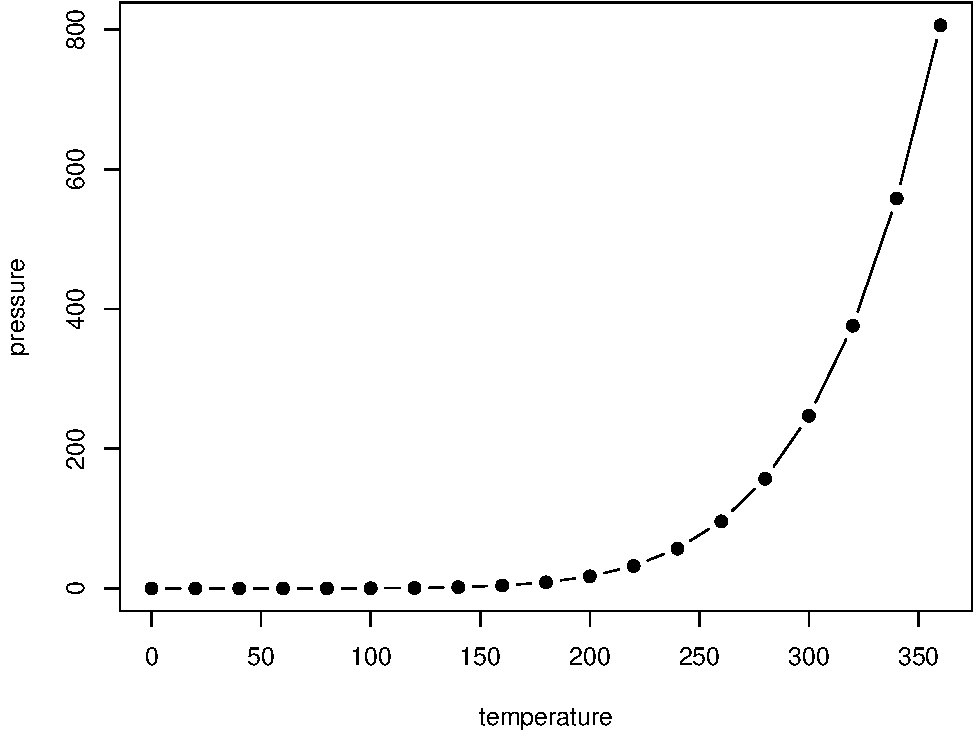
\includegraphics[width=0.8\linewidth]{01-theGolemOfPrague_files/figure-latex/nice-fig-1} 

}

\caption{Here is a nice figure!}\label{fig:nice-fig}
\end{figure}

Reference a figure by its code chunk label with the \texttt{fig:} prefix, e.g., see Figure \ref{fig:nice-fig}. Similarly, you can reference tables generated from \texttt{knitr::kable()}, e.g., see Table \ref{tab:nice-tab}.

\begin{Shaded}
\begin{Highlighting}[]
\NormalTok{knitr}\OperatorTok{::}\KeywordTok{kable}\NormalTok{(}
  \KeywordTok{head}\NormalTok{(iris, }\DecValTok{20}\NormalTok{), }\DataTypeTok{caption =} \StringTok{'Here is a nice table!'}\NormalTok{,}
  \DataTypeTok{booktabs =} \OtherTok{TRUE}
\NormalTok{)}
\end{Highlighting}
\end{Shaded}

\begin{table}

\caption{\label{tab:nice-tab}Here is a nice table!}
\centering
\begin{tabular}[t]{rrrrl}
\toprule
Sepal.Length & Sepal.Width & Petal.Length & Petal.Width & Species\\
\midrule
5.1 & 3.5 & 1.4 & 0.2 & setosa\\
4.9 & 3.0 & 1.4 & 0.2 & setosa\\
4.7 & 3.2 & 1.3 & 0.2 & setosa\\
4.6 & 3.1 & 1.5 & 0.2 & setosa\\
5.0 & 3.6 & 1.4 & 0.2 & setosa\\
\addlinespace
5.4 & 3.9 & 1.7 & 0.4 & setosa\\
4.6 & 3.4 & 1.4 & 0.3 & setosa\\
5.0 & 3.4 & 1.5 & 0.2 & setosa\\
4.4 & 2.9 & 1.4 & 0.2 & setosa\\
4.9 & 3.1 & 1.5 & 0.1 & setosa\\
\addlinespace
5.4 & 3.7 & 1.5 & 0.2 & setosa\\
4.8 & 3.4 & 1.6 & 0.2 & setosa\\
4.8 & 3.0 & 1.4 & 0.1 & setosa\\
4.3 & 3.0 & 1.1 & 0.1 & setosa\\
5.8 & 4.0 & 1.2 & 0.2 & setosa\\
\addlinespace
5.7 & 4.4 & 1.5 & 0.4 & setosa\\
5.4 & 3.9 & 1.3 & 0.4 & setosa\\
5.1 & 3.5 & 1.4 & 0.3 & setosa\\
5.7 & 3.8 & 1.7 & 0.3 & setosa\\
5.1 & 3.8 & 1.5 & 0.3 & setosa\\
\bottomrule
\end{tabular}
\end{table}

You can write citations, too. For example, we are using the \textbf{bookdown} package \citep{R-bookdown} in this sample book, which was built on top of R Markdown and \textbf{knitr} \citep{xie2015}.

\hypertarget{small-worlds-and-large-worlds}{%
\chapter{Small Worlds and Large Worlds}\label{small-worlds-and-large-worlds}}

Differentiate between the small world --- the self-contained logical world of the model --- and the large world --- the broader context in which one deploys a model. Statistical models pertain to the small world, and insofar as their assumptions reflect reality, they are useful in the large world. Bayesian learning is optimal in the small world in terms of how it makes use of information in the data, but that optimality only transfers to the large world inasmuch as the small world is an accurate description of the large world.

The small world is about probability theory and the stylized components of a Bayesian statistical model for learning from data.

We collect a sequence of observations --- data. Building a model involves making assumptions:

\begin{enumerate}
\def\labelenumi{\arabic{enumi}.}
\tightlist
\item
  Data story: how the data arise
\item
  Update: educate your model by feeding it data
\item
  Evaluate: supervise, critique and often rebuild.
\end{enumerate}

We need to name all the variables and define them. Variables are symbols that can take on different values. They can be unobserved variables (i.e.~parameters) or observed variables (things we can measure and use to infer the unobserved variable values).

\hypertarget{end-of-chapter-exercises}{%
\section{End of chapter exercises}\label{end-of-chapter-exercises}}

\hypertarget{h1.}{%
\subsection{2H1.}\label{h1.}}

Suppose there are two species of panda bear. Both are equally common in the wild and live in the same places. They look exactly alike and eat the same food, and there is yet no genetic assay capable of telling them apart. They differ however in their family sizes. Species A gives birth to twins \(10\%\) of the time, otherwise birthing a single infant. Species B births twins \(20%
\) of the time, otherwise birthing singleton infants. Assume these numbers are known with certainty, from many years of field research.

Now suppose you are managing a captive panda breeding program. You have a new female panda of unknown species, and she has just given birth to twins. What is the probability that her next birth will also be twins?

\textbf{Solution}

\begin{Shaded}
\begin{Highlighting}[]
\CommentTok{#2H1}
\NormalTok{prior =}\StringTok{ }\KeywordTok{c}\NormalTok{(}\FloatTok{0.5}\NormalTok{, }\FloatTok{0.5}\NormalTok{)}
\NormalTok{likelihood =}\StringTok{ }\KeywordTok{c}\NormalTok{(}\FloatTok{0.1}\NormalTok{, }\FloatTok{0.2}\NormalTok{)}
\NormalTok{posterior_unst =}\StringTok{ }\NormalTok{likelihood }\OperatorTok{*}\StringTok{ }\NormalTok{prior}
\NormalTok{posterior =}\StringTok{ }\NormalTok{posterior_unst }\OperatorTok{/}\StringTok{ }\KeywordTok{sum}\NormalTok{(posterior_unst)}
\CommentTok{# probability next birth is twins:}
\NormalTok{posterior[}\DecValTok{1}\NormalTok{] }\OperatorTok{*}\StringTok{ }\FloatTok{0.1} \OperatorTok{+}\StringTok{ }\NormalTok{posterior[}\DecValTok{2}\NormalTok{] }\OperatorTok{*}\StringTok{ }\FloatTok{0.2}
\end{Highlighting}
\end{Shaded}

\begin{verbatim}
## [1] 0.1666667
\end{verbatim}

\hypertarget{h2.}{%
\subsection{2H2.}\label{h2.}}

Recall all the facts from the problem above. Now compute the probability that the panda we have is from species A, assuming we have observed only the first birth and that it was twins.

\textbf{Solution}

\begin{Shaded}
\begin{Highlighting}[]
\CommentTok{# 2H2}
\NormalTok{prior1 =}\StringTok{ }\KeywordTok{c}\NormalTok{(}\FloatTok{0.5}\NormalTok{, }\FloatTok{0.5}\NormalTok{) }\CommentTok{# A, B}
\NormalTok{likelihood1 =}\StringTok{ }\KeywordTok{c}\NormalTok{(}\FloatTok{0.1}\NormalTok{, }\FloatTok{0.2}\NormalTok{) }\CommentTok{#A, B}
\NormalTok{posterior_unst1 =}\StringTok{ }\NormalTok{likelihood1 }\OperatorTok{*}\StringTok{ }\NormalTok{prior1}
\NormalTok{posterior1 =}\StringTok{ }\NormalTok{posterior_unst }\OperatorTok{/}\StringTok{ }\KeywordTok{sum}\NormalTok{(posterior_unst)}
\CommentTok{# probability she is species A}
\NormalTok{posterior1[}\DecValTok{1}\NormalTok{]}
\end{Highlighting}
\end{Shaded}

\begin{verbatim}
## [1] 0.3333333
\end{verbatim}

\begin{Shaded}
\begin{Highlighting}[]
\NormalTok{posterior1}
\end{Highlighting}
\end{Shaded}

\begin{verbatim}
## [1] 0.3333333 0.6666667
\end{verbatim}

\hypertarget{h3.}{%
\subsection{2H3.}\label{h3.}}

Continuing on from the previous problem, suppose the same panda mother has a second birth and that it is not twins, but a singleton infant. Compute the posterior probability that this panda is species A.
\textbf{Solution}
Want: \(P(\neg t2|t1,A)\).

\begin{Shaded}
\begin{Highlighting}[]
\CommentTok{# 2H3}
\NormalTok{prior2 =}\StringTok{ }\NormalTok{posterior1}
\NormalTok{likelihood2 =}\StringTok{ }\DecValTok{1} \OperatorTok{-}\StringTok{ }\NormalTok{likelihood1}
\NormalTok{posterior_unst2 =}\StringTok{ }\NormalTok{prior2 }\OperatorTok{*}\StringTok{ }\NormalTok{likelihood2}
\NormalTok{posterior2 =}\StringTok{ }\NormalTok{posterior_unst2 }\OperatorTok{/}\StringTok{ }\KeywordTok{sum}\NormalTok{(posterior_unst2)}
\NormalTok{posterior2}
\end{Highlighting}
\end{Shaded}

\begin{verbatim}
## [1] 0.36 0.64
\end{verbatim}

\begin{Shaded}
\begin{Highlighting}[]
\CommentTok{# Prob of singleton given species A and twins}
\NormalTok{posterior2[}\DecValTok{1}\NormalTok{]}
\end{Highlighting}
\end{Shaded}

\begin{verbatim}
## [1] 0.36
\end{verbatim}

\begin{Shaded}
\begin{Highlighting}[]
\NormalTok{pr =}\StringTok{ }\KeywordTok{c}\NormalTok{(}\FloatTok{0.5}\NormalTok{, }\FloatTok{0.5}\NormalTok{)}
\NormalTok{lik =}\StringTok{ }\KeywordTok{c}\NormalTok{(}\FloatTok{0.1}\OperatorTok{*}\FloatTok{0.9}\NormalTok{, }\FloatTok{0.2}\OperatorTok{*}\FloatTok{0.8}\NormalTok{)}
\NormalTok{po =}\StringTok{ }\NormalTok{pr }\OperatorTok{*}\StringTok{ }\NormalTok{lik}
\NormalTok{po =}\StringTok{ }\NormalTok{po}\OperatorTok{/}\KeywordTok{sum}\NormalTok{(po)}
\NormalTok{po}
\end{Highlighting}
\end{Shaded}

\begin{verbatim}
## [1] 0.36 0.64
\end{verbatim}

\hypertarget{h4.}{%
\subsection{2H4.}\label{h4.}}

A common boast of Bayesian statisticians is that Bayesian inference makes it easy to use all of the data, even if the data are of different types.

So suppose now that a veterinarian comes along who has a new genetic test that she claims can identify the species of our mother panda. But the test, like all tests, is imperfect. This is the information you have about the test:

\begin{itemize}
\tightlist
\item
  The probability it correctly identifies a species A panda is 0.8.
\item
  The probability it correctly identifies a species B panda is 0.65.
\end{itemize}

The vet administers the test to your panda and tells you that the test is positive for species A. First ignore your previous information from the births and compute the posterior probability that your panda is species A. Then redo your calculation, now using the birth data as well.

\textbf{Solution}
Know: \(P(testA|A) = 0.8\) and \(P(testB|B)=0.65\), and can infer \(P(testA|B)=1-0.65 = 0.35\) and \(P(testB|A) = 1-0.8 = 0.2\).

Want: \(P(A|testA) = \frac{P(testA|A)P(A)}{P(testA)}\)

\[
\begin{aligned}
P(testA) &= P(testA|A)P(A) + P(testA|B)P(B) \\
&= 0.8\times0.5 + 0.35\times 0.5 \\
&= 0.575
\end{aligned}
\]

\begin{Shaded}
\begin{Highlighting}[]
\CommentTok{# 2H4}
\CommentTok{# No birth information}
\NormalTok{prior3 =}\StringTok{ }\KeywordTok{c}\NormalTok{(}\FloatTok{0.5}\NormalTok{, }\FloatTok{0.5}\NormalTok{)}
\NormalTok{likelihood3 =}\StringTok{ }\KeywordTok{c}\NormalTok{(}\FloatTok{0.8}\NormalTok{, }\FloatTok{0.35}\NormalTok{)}
\NormalTok{posterior_unst3 =}\StringTok{ }\NormalTok{prior3 }\OperatorTok{*}\StringTok{ }\NormalTok{likelihood3}
\NormalTok{posterior3 =}\StringTok{ }\NormalTok{posterior_unst3 }\OperatorTok{/}\StringTok{ }\KeywordTok{sum}\NormalTok{(posterior_unst3)}
\NormalTok{posterior3 }
\end{Highlighting}
\end{Shaded}

\begin{verbatim}
## [1] 0.6956522 0.3043478
\end{verbatim}

\begin{Shaded}
\begin{Highlighting}[]
\CommentTok{# Birth information}
\NormalTok{prior4 =}\StringTok{ }\NormalTok{posterior2}
\NormalTok{likelihood4 =}\StringTok{ }\KeywordTok{c}\NormalTok{(}\FloatTok{0.8}\NormalTok{, }\FloatTok{0.35}\NormalTok{)}
\NormalTok{posterior_unst4 =}\StringTok{ }\NormalTok{prior4 }\OperatorTok{*}\StringTok{ }\NormalTok{likelihood4}
\NormalTok{posterior4 =}\StringTok{ }\NormalTok{posterior_unst4 }\OperatorTok{/}\StringTok{ }\KeywordTok{sum}\NormalTok{(posterior_unst4)}
\NormalTok{posterior4 }
\end{Highlighting}
\end{Shaded}

\begin{verbatim}
## [1] 0.5625 0.4375
\end{verbatim}

\hypertarget{sampling-the-imaginary}{%
\chapter{Sampling the imaginary}\label{sampling-the-imaginary}}

There is a blood test that correctly detects vampirism \(95\%\) of the time and incorrectly diagnoses normal people as vampires \(1\%\) of the time. Letting \(v\) denote being a vampire and \(h\) denote being human (not vampire) and \(+\) denote testing positive for vampirism, and \(-\) denote testing negative for vampirism, then we have:
\[
\begin{aligned}
\mathbb P(+|v) &= 0.95 \\
\mathbb P(-|v) &= 0.05 \\
\mathbb P(+|h) &= 0.01 \\
\mathbb P(-|h) &= 0.99 \\
\end{aligned}
\]
Suppose that vampires are quite rare, comprising only \(0.1\%\) of the population. That is \(\mathbb P(v) = 0.001\).

Now suppose someone tests positive for vampirism. What's the actual probability that he/she is really a vampire?

Using Bayes' theorem this is simple. We want \(\mathbb P(v|+)\) and we can find it through probability inversion as follows:
\[
\begin{aligned}
\mathbb P(v|+) &= \frac{\mathbb P(+|v) \mathbb P(v)}{P(+)} \\
&= \frac{\mathbb P(+|v) \mathbb P(v)}{\mathbb P(+|v)\mathbb P(v) + \mathbb P(+|h)\mathbb P(h)} \\
&= \frac{0.95\times 0.001}{0.95\times 0.001 + 0.01 \times 0.999} \\
&= 0.08683729
\end{aligned}
\]
The calculations can be carried out easily in R:

\begin{Shaded}
\begin{Highlighting}[]
\NormalTok{p_pos_v =}\StringTok{ }\FloatTok{0.95}
\NormalTok{p_pos_h =}\StringTok{ }\FloatTok{0.01}
\NormalTok{p_neg_v =}\StringTok{ }\DecValTok{1} \OperatorTok{-}\StringTok{ }\NormalTok{p_pos_v}
\NormalTok{p_neg_h =}\StringTok{ }\DecValTok{1} \OperatorTok{-}\StringTok{ }\NormalTok{p_pos_h}
\NormalTok{p_v =}\StringTok{ }\FloatTok{0.001}
\NormalTok{p_h =}\StringTok{ }\DecValTok{1} \OperatorTok{-}\StringTok{ }\NormalTok{p_v}

\NormalTok{p_pos =}\StringTok{ }\NormalTok{p_pos_v }\OperatorTok{*}\StringTok{ }\NormalTok{p_v }\OperatorTok{+}\StringTok{ }\NormalTok{p_pos_h }\OperatorTok{*}\StringTok{ }\NormalTok{p_h }
\NormalTok{p_v_pos =}\StringTok{ }\NormalTok{p_pos_v }\OperatorTok{*}\StringTok{ }\NormalTok{p_v }\OperatorTok{/}\StringTok{ }\NormalTok{p_pos}

\KeywordTok{print}\NormalTok{(p_v_pos)}
\end{Highlighting}
\end{Shaded}

\begin{verbatim}
## [1] 0.08683729
\end{verbatim}

There is (only) an \(8.7\%\) that the tested person is actually a vampire. Whenever the condition of interest is very rare, having a test that finds all the true cases is still no guarantee that a positive result carries much information at all. Why? Because most positive tests are false positives, even when all the true positives are detected correctly.

The above results seems counter-intuitive. But there's a way to frame it --- in terms of frequencies --- that makes it far easier. Suppose we have 100000 people in the population and 100 of them are vampires. Of the 100 vampires, 95 of them would test positive for vampirism. Of the 99900 humans, 999 of them would test positive for vampirism.

Now, suppose we test the whole population, what proportion of those who test positive do you expect to actually be vampires? It's simple now right:
\[
\mathbb P(v|+) = \frac{95}{1094} \approx 0.087
\]
Using frequencies makes things easier --- and we exploit this fact when we sample from a posterior distribution.

\hypertarget{sampling-from-a-grid-approximate-posterior}{%
\section{Sampling from a grid-approximate posterior}\label{sampling-from-a-grid-approximate-posterior}}

A globe-tossing model: You have a globe representing Earth and you're curious about how much of the surface is covered in water. You will toss the globe in the air and catch it, and record whether or not the surface under your right index finger is water or land. Repeat the procedure some number of times and then look at the relative proportions of water to land. The first 9 observations are
\[
W\;L\;W\;W\;W\;L\;W\;L\;W
\]
Before we can work with samples, we need to generate them.

The data story is simply that the true proportion of water covering the globe is \(p\), a single toss of the globe has probability \(p\) of producing water and probability \(1-p\) of producing land, and each toss of the globe is independent of the others.

To translate the data story into a probability model: the counts of ``water'' and ``land'' are distributed binomially, with probability \(p\) of water on each toss:
\[
\mathbb P(W,L|p) = \frac{(W+L)!}{W!L!}p^W(1-p)^L.
\]
A Bayesian model specifies a likelihood:
\[
W \sim \text{Binomial}(N,p); \quad N = W + L
\]
and a prior:
\[
p \sim \text{Uniform}(0,1)
\]
To actually process the data and model, to produce a posterior, we need an engine. Most real-world models don't allow us to find analytical (pen and paper) solutions. Instead for small models we can use grid approximation, for moderately larger models we canuse quadratic approximation, and for proper real-world models we can use MCMC.

\begin{Shaded}
\begin{Highlighting}[]
\ControlFlowTok{if}\NormalTok{(}\OperatorTok{!}\KeywordTok{require}\NormalTok{(pacman)) }\KeywordTok{install.packages}\NormalTok{(pacman)}
\end{Highlighting}
\end{Shaded}

\begin{verbatim}
## Loading required package: pacman
\end{verbatim}

\begin{Shaded}
\begin{Highlighting}[]
\KeywordTok{library}\NormalTok{(pacman)}
\end{Highlighting}
\end{Shaded}

\begin{Shaded}
\begin{Highlighting}[]
\NormalTok{n_grid =}\StringTok{ }\DecValTok{1000}
\NormalTok{grid_limits =}\StringTok{ }\KeywordTok{c}\NormalTok{(}\DecValTok{0}\NormalTok{,}\DecValTok{1}\NormalTok{)}
\NormalTok{p_grid =}\StringTok{ }\KeywordTok{seq}\NormalTok{( }\DataTypeTok{from=}\NormalTok{grid_limits[}\DecValTok{1}\NormalTok{], }\DataTypeTok{to=}\NormalTok{grid_limits[}\DecValTok{2}\NormalTok{], }\DataTypeTok{length.out=}\NormalTok{n_grid)}
\NormalTok{prob_p =}\StringTok{ }\KeywordTok{rep}\NormalTok{( }\DecValTok{1}\NormalTok{, }\DecValTok{1000}\NormalTok{)}
\NormalTok{prob_data =}\StringTok{ }\KeywordTok{dbinom}\NormalTok{( }\DecValTok{6}\NormalTok{, }\DataTypeTok{size=}\DecValTok{9}\NormalTok{, }\DataTypeTok{prob=}\NormalTok{p_grid )}
\NormalTok{posterior =}\StringTok{ }\NormalTok{prob_data }\OperatorTok{*}\StringTok{ }\NormalTok{prob_p}
\NormalTok{posterior =}\StringTok{ }\NormalTok{posterior }\OperatorTok{/}\StringTok{ }\KeywordTok{sum}\NormalTok{(posterior)}
\end{Highlighting}
\end{Shaded}

\begin{Shaded}
\begin{Highlighting}[]
\NormalTok{pacman}\OperatorTok{::}\KeywordTok{p_load}\NormalTok{(rethinking)}

\NormalTok{samples =}\StringTok{ }\KeywordTok{sample}\NormalTok{( p_grid, }\DataTypeTok{prob=}\NormalTok{posterior, }\DataTypeTok{size=}\FloatTok{1e4}\NormalTok{, }\DataTypeTok{replace=}\OtherTok{TRUE}\NormalTok{ )}
\KeywordTok{plot}\NormalTok{( samples )}
\end{Highlighting}
\end{Shaded}

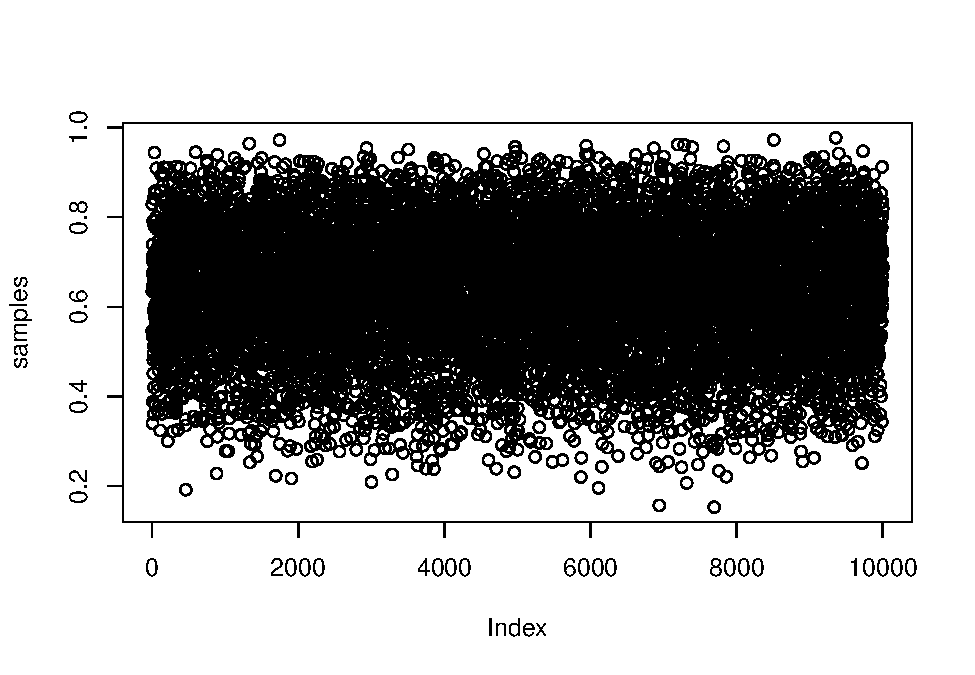
\includegraphics{03-samplingTheImaginary_files/figure-latex/unnamed-chunk-4-1.pdf}

\begin{Shaded}
\begin{Highlighting}[]
\KeywordTok{dens}\NormalTok{( samples )}
\end{Highlighting}
\end{Shaded}

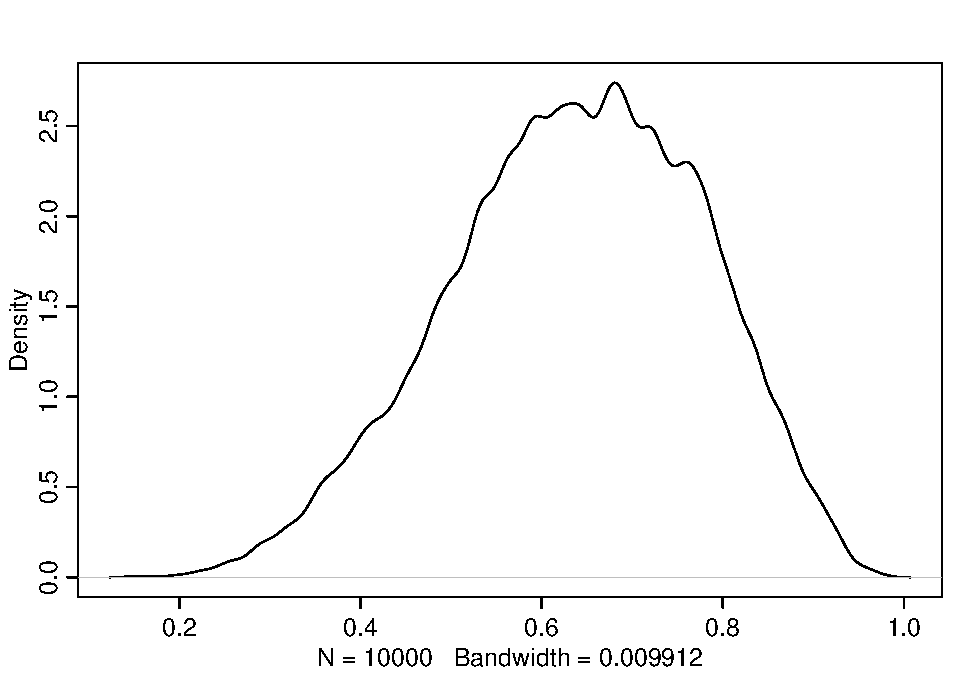
\includegraphics{03-samplingTheImaginary_files/figure-latex/unnamed-chunk-4-2.pdf}
\#\# Sampling to summarize

\hypertarget{intervals-of-defined-boundaries}{%
\subsection{Intervals of defined boundaries}\label{intervals-of-defined-boundaries}}

To get the proportion of water less than some value of \texttt{p\_grid}:

\begin{Shaded}
\begin{Highlighting}[]
\KeywordTok{sum}\NormalTok{( samples }\OperatorTok{<}\StringTok{ }\FloatTok{0.5}\NormalTok{ ) }\OperatorTok{/}\StringTok{ }\FloatTok{1e4}
\end{Highlighting}
\end{Shaded}

\begin{verbatim}
## [1] 0.1706
\end{verbatim}

\begin{Shaded}
\begin{Highlighting}[]
\KeywordTok{sum}\NormalTok{( samples }\OperatorTok{>}\StringTok{ }\FloatTok{0.5} \OperatorTok{&}\StringTok{ }\NormalTok{samples }\OperatorTok{<}\StringTok{ }\FloatTok{0.75}\NormalTok{ ) }\OperatorTok{/}\StringTok{ }\FloatTok{1e4}
\end{Highlighting}
\end{Shaded}

\begin{verbatim}
## [1] 0.5998
\end{verbatim}

\begin{Shaded}
\begin{Highlighting}[]
\KeywordTok{quantile}\NormalTok{( samples, }\FloatTok{0.8}\NormalTok{)}
\end{Highlighting}
\end{Shaded}

\begin{verbatim}
##       80% 
## 0.7627628
\end{verbatim}

\begin{Shaded}
\begin{Highlighting}[]
\KeywordTok{quantile}\NormalTok{( samples, }\KeywordTok{c}\NormalTok{(}\FloatTok{0.1}\NormalTok{, }\FloatTok{0.9}\NormalTok{) )}
\end{Highlighting}
\end{Shaded}

\begin{verbatim}
##       10%       90% 
## 0.4494494 0.8128128
\end{verbatim}

\begin{Shaded}
\begin{Highlighting}[]
\NormalTok{n_grid =}\StringTok{ }\DecValTok{1000}
\NormalTok{grid_limits =}\StringTok{ }\KeywordTok{c}\NormalTok{(}\DecValTok{0}\NormalTok{,}\DecValTok{1}\NormalTok{)}
\NormalTok{p_grid =}\StringTok{ }\KeywordTok{seq}\NormalTok{( }\DataTypeTok{from=}\NormalTok{grid_limits[}\DecValTok{1}\NormalTok{], }\DataTypeTok{to=}\NormalTok{grid_limits[}\DecValTok{2}\NormalTok{], }\DataTypeTok{length.out=}\NormalTok{n_grid)}
\NormalTok{prior =}\StringTok{ }\KeywordTok{rep}\NormalTok{( }\DecValTok{1}\NormalTok{, n_grid)}
\NormalTok{likelihood =}\StringTok{ }\KeywordTok{dbinom}\NormalTok{( }\DecValTok{3}\NormalTok{, }\DataTypeTok{size=}\DecValTok{3}\NormalTok{, }\DataTypeTok{prob=}\NormalTok{p_grid )}
\NormalTok{posterior =}\StringTok{ }\NormalTok{likelihood }\OperatorTok{*}\StringTok{ }\NormalTok{prior}
\NormalTok{posterior =}\StringTok{ }\NormalTok{posterior }\OperatorTok{/}\StringTok{ }\KeywordTok{sum}\NormalTok{(posterior)}
\NormalTok{samples =}\StringTok{ }\KeywordTok{sample}\NormalTok{( p_grid, }\DataTypeTok{size=}\FloatTok{1e4}\NormalTok{, }\DataTypeTok{replace=}\OtherTok{TRUE}\NormalTok{, }\DataTypeTok{prob=}\NormalTok{posterior )}
\end{Highlighting}
\end{Shaded}

\begin{Shaded}
\begin{Highlighting}[]
\KeywordTok{PI}\NormalTok{( samples, }\DataTypeTok{prob=}\FloatTok{0.5}\NormalTok{ )}
\end{Highlighting}
\end{Shaded}

\begin{verbatim}
##       25%       75% 
## 0.7027027 0.9319319
\end{verbatim}

\begin{Shaded}
\begin{Highlighting}[]
\KeywordTok{HPDI}\NormalTok{( samples, }\DataTypeTok{prob=}\FloatTok{0.5}\NormalTok{ )}
\end{Highlighting}
\end{Shaded}

\begin{verbatim}
##      |0.5      0.5| 
## 0.8428428 1.0000000
\end{verbatim}

\begin{Shaded}
\begin{Highlighting}[]
\NormalTok{p_grid[ }\KeywordTok{which.max}\NormalTok{(posterior) ]}
\end{Highlighting}
\end{Shaded}

\begin{verbatim}
## [1] 1
\end{verbatim}

\begin{Shaded}
\begin{Highlighting}[]
\KeywordTok{chainmode}\NormalTok{( samples, }\DataTypeTok{adj=}\FloatTok{0.01}\NormalTok{ )}
\end{Highlighting}
\end{Shaded}

\begin{verbatim}
## [1] 0.9972145
\end{verbatim}

\begin{Shaded}
\begin{Highlighting}[]
\KeywordTok{mean}\NormalTok{( samples )}
\end{Highlighting}
\end{Shaded}

\begin{verbatim}
## [1] 0.8001998
\end{verbatim}

\begin{Shaded}
\begin{Highlighting}[]
\KeywordTok{median}\NormalTok{( samples )}
\end{Highlighting}
\end{Shaded}

\begin{verbatim}
## [1] 0.8428428
\end{verbatim}

\begin{Shaded}
\begin{Highlighting}[]
\KeywordTok{sum}\NormalTok{( posterior }\OperatorTok{*}\StringTok{ }\KeywordTok{abs}\NormalTok{( }\FloatTok{0.5} \OperatorTok{-}\StringTok{ }\NormalTok{p_grid ) )}
\end{Highlighting}
\end{Shaded}

\begin{verbatim}
## [1] 0.3128752
\end{verbatim}

\begin{Shaded}
\begin{Highlighting}[]
\NormalTok{pacman}\OperatorTok{::}\KeywordTok{p_load}\NormalTok{(purrr)}

\NormalTok{loss =}\StringTok{ }\KeywordTok{map_dbl}\NormalTok{( }
\NormalTok{    p_grid, }
    \ControlFlowTok{function}\NormalTok{(d)\{ }\KeywordTok{sum}\NormalTok{( posterior }\OperatorTok{*}\StringTok{ }\KeywordTok{abs}\NormalTok{( d }\OperatorTok{-}\StringTok{ }\NormalTok{p_grid ) ) \} )}

\NormalTok{p_grid[ }\KeywordTok{which.min}\NormalTok{(loss) ]}
\end{Highlighting}
\end{Shaded}

\begin{verbatim}
## [1] 0.8408408
\end{verbatim}

Generating dummy data: suppose we have two tosses and the probability of water is 0.7: \((N=2, p = 0.7)\). To compute the probability of the possible outcomes:

\begin{Shaded}
\begin{Highlighting}[]
\NormalTok{N =}\StringTok{ }\DecValTok{9}
\NormalTok{p =}\StringTok{ }\FloatTok{0.7}
\NormalTok{w =}\StringTok{ }\DecValTok{0}\OperatorTok{:}\NormalTok{N}
\NormalTok{probs =}\StringTok{ }\KeywordTok{dbinom}\NormalTok{( w, }\DataTypeTok{size=}\NormalTok{N, }\DataTypeTok{prob=}\NormalTok{p)}
\end{Highlighting}
\end{Shaded}

This tells us that there is a \(9\%\) chance that \(w=0\), a \(42\%\) chance that \(w=1\) and a \(49\%\) chance that \(w=2\).

Let's simulate observations now using these probabilities:

\begin{Shaded}
\begin{Highlighting}[]
\NormalTok{n_samples =}\StringTok{ }\FloatTok{1e6}
\NormalTok{dummy_w =}\StringTok{ }\KeywordTok{rbinom}\NormalTok{(n_samples, }\DataTypeTok{size=}\NormalTok{N, }\DataTypeTok{prob=}\NormalTok{p )}
\KeywordTok{table}\NormalTok{(dummy_w)}\OperatorTok{/}\NormalTok{n_samples}
\end{Highlighting}
\end{Shaded}

\begin{verbatim}
## dummy_w
##        0        1        2        3        4        5        6        7 
## 0.000018 0.000431 0.003869 0.021115 0.073042 0.172010 0.266576 0.267091 
##        8        9 
## 0.155379 0.040469
\end{verbatim}

\begin{Shaded}
\begin{Highlighting}[]
\KeywordTok{simplehist}\NormalTok{( dummy_w, }\DataTypeTok{xlab=}\StringTok{"dummy water count"}\NormalTok{ )}
\end{Highlighting}
\end{Shaded}

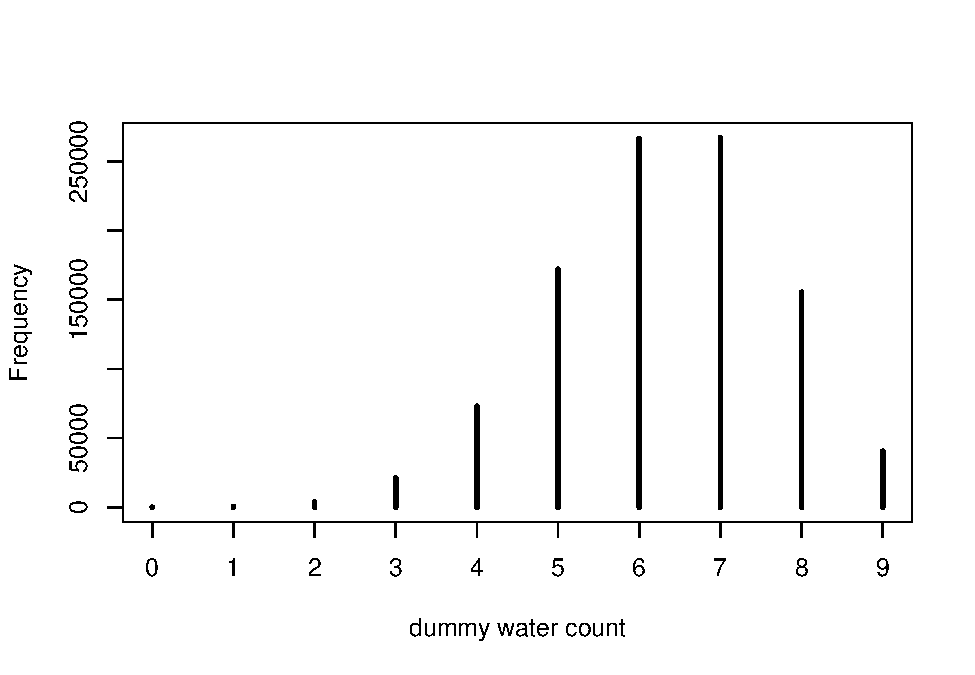
\includegraphics{03-samplingTheImaginary_files/figure-latex/unnamed-chunk-10-1.pdf}

\begin{Shaded}
\begin{Highlighting}[]
\NormalTok{w =}\StringTok{ }\KeywordTok{rbinom}\NormalTok{( n_samples, }\DataTypeTok{size=}\NormalTok{N, }\DataTypeTok{prob=}\NormalTok{samples)}
\KeywordTok{simplehist}\NormalTok{(w)}
\end{Highlighting}
\end{Shaded}

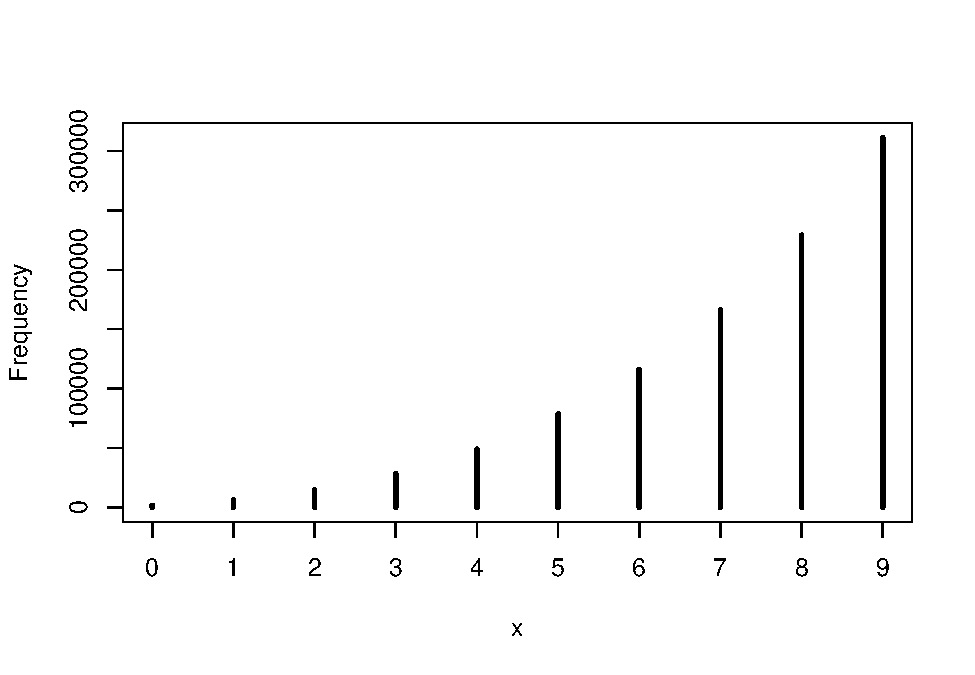
\includegraphics{03-samplingTheImaginary_files/figure-latex/unnamed-chunk-11-1.pdf}

\hypertarget{chapter-3-practice-problems}{%
\section{Chapter 3 Practice Problems}\label{chapter-3-practice-problems}}

The easy problems all use the following code:

\begin{Shaded}
\begin{Highlighting}[]
\KeywordTok{require}\NormalTok{(rethinking)}
\NormalTok{p_grid <-}\StringTok{ }\KeywordTok{seq}\NormalTok{( }\DataTypeTok{from=}\DecValTok{0}\NormalTok{, }\DataTypeTok{to=}\DecValTok{1}\NormalTok{, }\DataTypeTok{length.out=}\DecValTok{1000}\NormalTok{)  }
\NormalTok{prior <-}\StringTok{ }\KeywordTok{rep}\NormalTok{( }\DecValTok{1}\NormalTok{, }\DecValTok{1000}\NormalTok{)  }
\NormalTok{likelihood <-}\StringTok{ }\KeywordTok{dbinom}\NormalTok{( }\DecValTok{6}\NormalTok{, }\DataTypeTok{size=}\DecValTok{9}\NormalTok{, }\DataTypeTok{prob=}\NormalTok{p_grid)  }
\NormalTok{posterior <-}\StringTok{ }\NormalTok{likelihood }\OperatorTok{*}\StringTok{ }\NormalTok{prior  }
\NormalTok{posterior <-}\StringTok{ }\NormalTok{posterior}\OperatorTok{/}\StringTok{ }\KeywordTok{sum}\NormalTok{(posterior) }
\KeywordTok{set.seed}\NormalTok{(}\DecValTok{100}\NormalTok{)}
\NormalTok{samples <-}\StringTok{ }\KeywordTok{sample}\NormalTok{(p_grid, }\DataTypeTok{prob=}\NormalTok{posterior, }\DataTypeTok{size=}\FloatTok{1e4}\NormalTok{, }\DataTypeTok{replace=}\OtherTok{TRUE}\NormalTok{)}
\KeywordTok{dens}\NormalTok{(samples)}
\end{Highlighting}
\end{Shaded}

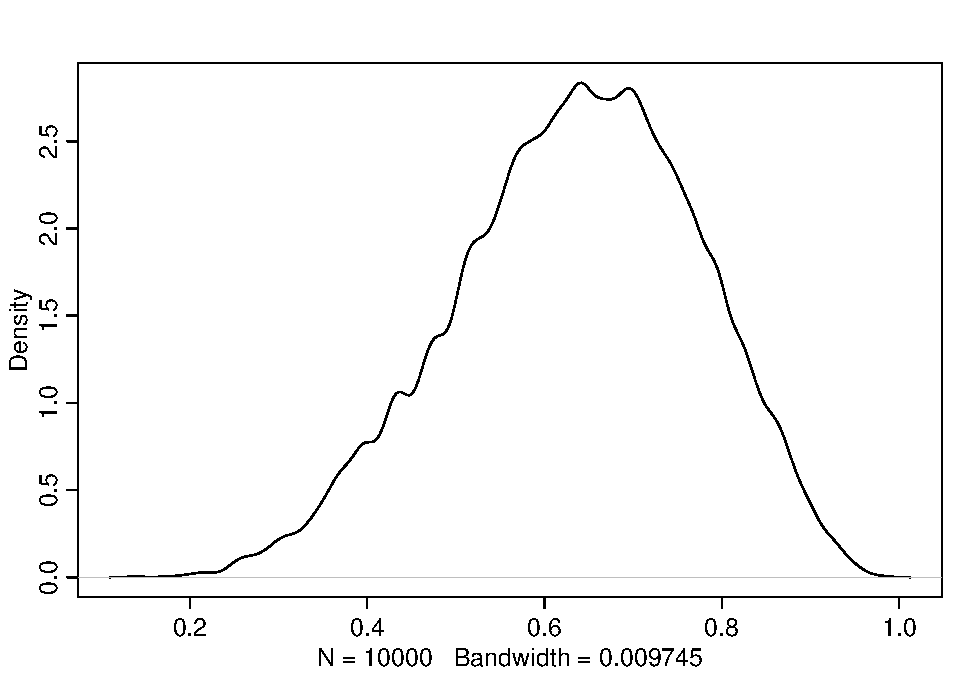
\includegraphics{03-samplingTheImaginary_files/figure-latex/unnamed-chunk-12-1.pdf}
Use the values in \texttt{samples} to answer the following questions:

\hypertarget{e1.}{%
\subsection{3E1.}\label{e1.}}

How much posterior probability lies below p = 0.2?

\textbf{Solution}
This is just asking for the sum of probabilities \(<0.2\):

\begin{Shaded}
\begin{Highlighting}[]
\CommentTok{# Using samples from posterior}
\NormalTok{sp =}\StringTok{ }\DecValTok{100} \OperatorTok{*}\StringTok{ }\KeywordTok{sum}\NormalTok{( samples }\OperatorTok{<}\StringTok{ }\FloatTok{0.2}\NormalTok{ ) }\OperatorTok{/}\StringTok{ }\FloatTok{1e4}

\CommentTok{# cf. grid-approximate posterior}
\NormalTok{gp =}\StringTok{ }\DecValTok{100} \OperatorTok{*}\StringTok{ }\KeywordTok{sum}\NormalTok{( posterior[ p_grid }\OperatorTok{<}\StringTok{ }\FloatTok{0.2}\NormalTok{ ])}

\KeywordTok{paste}\NormalTok{(}\StringTok{"The samples give "}\NormalTok{, }\KeywordTok{round}\NormalTok{(sp,}\DecValTok{4}\NormalTok{), }\StringTok{"% less than 0.2, while the grid-approximate posterior indicates "}\NormalTok{, }\KeywordTok{round}\NormalTok{(gp,}\DecValTok{4}\NormalTok{), }\StringTok{"% less than 0.2"}\NormalTok{)}
\end{Highlighting}
\end{Shaded}

\begin{verbatim}
## [1] "The samples give  0.04 % less than 0.2, while the grid-approximate posterior indicates  0.0856 % less than 0.2"
\end{verbatim}

\hypertarget{e2.}{%
\subsection{3E2.}\label{e2.}}

How much posterior probability lies above p = 0.8?

\textbf{Solution}
This is just asking for the sum of probabilities on \(> 0.8\)

\begin{Shaded}
\begin{Highlighting}[]
\CommentTok{# Using samples from posterior}
\NormalTok{sp =}\StringTok{ }\DecValTok{100} \OperatorTok{*}\StringTok{ }\KeywordTok{sum}\NormalTok{( samples }\OperatorTok{>}\StringTok{ }\FloatTok{0.8}\NormalTok{ ) }\OperatorTok{/}\StringTok{ }\FloatTok{1e4}

\CommentTok{# cf. grid-approximate posterior}
\NormalTok{gp =}\StringTok{ }\DecValTok{100} \OperatorTok{*}\StringTok{ }\KeywordTok{sum}\NormalTok{( posterior[ p_grid }\OperatorTok{>}\StringTok{ }\FloatTok{0.8}\NormalTok{ ])}

\KeywordTok{paste}\NormalTok{(}\StringTok{"The samples give "}\NormalTok{, }\KeywordTok{round}\NormalTok{(sp,}\DecValTok{4}\NormalTok{), }\StringTok{"% greater than 0.8, while the grid-approximate posterior indicates "}\NormalTok{, }\KeywordTok{round}\NormalTok{(gp,}\DecValTok{4}\NormalTok{), }\StringTok{"% greater than 0.8"}\NormalTok{)}
\end{Highlighting}
\end{Shaded}

\begin{verbatim}
## [1] "The samples give  11.16 % greater than 0.8, while the grid-approximate posterior indicates  12.0345 % greater than 0.8"
\end{verbatim}

\hypertarget{e3.}{%
\subsection{3E3.}\label{e3.}}

How much posterior probability lies between p = 0.2 and p = 0.8?

\textbf{Solution}
This is just asking for the sum of probabilities on \(> 0.2\; \&\; <0.8\)

\begin{Shaded}
\begin{Highlighting}[]
\CommentTok{# samples}
\NormalTok{sp =}\StringTok{ }\DecValTok{100} \OperatorTok{*}\StringTok{ }\KeywordTok{sum}\NormalTok{( samples }\OperatorTok{>}\StringTok{ }\FloatTok{0.2} \OperatorTok{&}\StringTok{ }\NormalTok{samples }\OperatorTok{<}\StringTok{ }\FloatTok{0.8}\NormalTok{) }\OperatorTok{/}\StringTok{ }\FloatTok{1e4}

\CommentTok{# grid-approximate}
\NormalTok{gp =}\StringTok{ }\DecValTok{100} \OperatorTok{*}\StringTok{ }\KeywordTok{sum}\NormalTok{( posterior[ p_grid }\OperatorTok{>}\StringTok{ }\FloatTok{0.2} \OperatorTok{&}\StringTok{ }\NormalTok{p_grid }\OperatorTok{<}\StringTok{ }\FloatTok{0.8}\NormalTok{ ])}

\KeywordTok{paste}\NormalTok{(}\StringTok{"The samples give"}\NormalTok{, }\KeywordTok{round}\NormalTok{(sp,}\DecValTok{4}\NormalTok{), }\StringTok{"% in (0.2, 0.8), while the grid-approximate posterior indicates"}\NormalTok{, }\KeywordTok{round}\NormalTok{(gp,}\DecValTok{4}\NormalTok{), }\StringTok{"% in (0.2, 0.8)"}\NormalTok{)}
\end{Highlighting}
\end{Shaded}

\begin{verbatim}
## [1] "The samples give 88.8 % in (0.2, 0.8), while the grid-approximate posterior indicates 87.8799 % in (0.2, 0.8)"
\end{verbatim}

\hypertarget{e4.}{%
\subsection{3E4.}\label{e4.}}

20\% of the posterior probability lies below which value of p?

\textbf{Solution}
This is just asking for the 20th percentile:

\begin{Shaded}
\begin{Highlighting}[]
\NormalTok{q_}\DecValTok{20}\NormalTok{ =}\StringTok{ }\KeywordTok{quantile}\NormalTok{( samples, }\FloatTok{0.2}\NormalTok{, }\DataTypeTok{lower.tail=}\OtherTok{TRUE}\NormalTok{)}

\KeywordTok{paste}\NormalTok{(}\StringTok{"The 20th percentile is"}\NormalTok{, }\KeywordTok{round}\NormalTok{(q_}\DecValTok{20}\NormalTok{, }\DecValTok{2}\NormalTok{), }\StringTok{"(to 2 dp)"}\NormalTok{) }
\end{Highlighting}
\end{Shaded}

\begin{verbatim}
## [1] "The 20th percentile is 0.52 (to 2 dp)"
\end{verbatim}

\hypertarget{e5.}{%
\subsection{3E5.}\label{e5.}}

20\% of the posterior probability lies above which value of p?

\textbf{Solution}
This is just asking for the (100 - 20)th = 80th percentile:

\begin{Shaded}
\begin{Highlighting}[]
\CommentTok{# from lower tail}
\NormalTok{q_}\DecValTok{80}\NormalTok{ =}\StringTok{ }\KeywordTok{quantile}\NormalTok{( samples, }\FloatTok{0.8}\NormalTok{, }\DataTypeTok{lower.tail=}\OtherTok{TRUE}\NormalTok{ )}

\KeywordTok{paste}\NormalTok{(}\StringTok{"The 80th percentile is"}\NormalTok{, }\KeywordTok{round}\NormalTok{(q_}\DecValTok{80}\NormalTok{, }\DecValTok{2}\NormalTok{), }\StringTok{"(to 2 dp)"}\NormalTok{) }
\end{Highlighting}
\end{Shaded}

\begin{verbatim}
## [1] "The 80th percentile is 0.76 (to 2 dp)"
\end{verbatim}

\hypertarget{e6.}{%
\subsection{3E6.}\label{e6.}}

Which values of p contain the narrowest interval equal to 66\% of the posterior probability?

\textbf{Solution}
This is just asking for the 66\% HPDI:

\begin{Shaded}
\begin{Highlighting}[]
\KeywordTok{require}\NormalTok{(rethinking)}
\NormalTok{HPDI_}\DecValTok{66}\NormalTok{ =}\StringTok{ }\KeywordTok{round}\NormalTok{( }\KeywordTok{HPDI}\NormalTok{( samples, }\DataTypeTok{prob=}\FloatTok{0.66}\NormalTok{ ), }\DecValTok{2}\NormalTok{)}
\NormalTok{HPDI_}\DecValTok{66}
\end{Highlighting}
\end{Shaded}

\begin{verbatim}
## |0.66 0.66| 
##  0.51  0.77
\end{verbatim}

\begin{Shaded}
\begin{Highlighting}[]
\KeywordTok{paste}\NormalTok{(}\StringTok{"The narrowest interval containing 66% of the probabilitiy mass is the 66% HPDI: "}\NormalTok{, }\StringTok{"["}\NormalTok{, HPDI_}\DecValTok{66}\NormalTok{[}\DecValTok{1}\NormalTok{],}\StringTok{","}\NormalTok{,HPDI_}\DecValTok{66}\NormalTok{[}\DecValTok{2}\NormalTok{], }\StringTok{"]"}\NormalTok{, }\StringTok{", (to 2 dp)"}\NormalTok{, }\DataTypeTok{sep=}\StringTok{""}\NormalTok{) }
\end{Highlighting}
\end{Shaded}

\begin{verbatim}
## [1] "The narrowest interval containing 66% of the probabilitiy mass is the 66% HPDI: [0.51,0.77], (to 2 dp)"
\end{verbatim}

\hypertarget{e7.}{%
\subsection{3E7.}\label{e7.}}

Which values of p contain 66\% of the posterior probability, assuming equal posterior probability both below and above the interval?

\textbf{Solution}
This is just asking for the 66\% PI:

\begin{Shaded}
\begin{Highlighting}[]
\KeywordTok{require}\NormalTok{(rethinking)}
\NormalTok{PI_}\DecValTok{66}\NormalTok{ =}\StringTok{ }\KeywordTok{round}\NormalTok{( }\KeywordTok{PI}\NormalTok{( samples, }\DataTypeTok{prob=}\FloatTok{0.66}\NormalTok{ ), }\DecValTok{2}\NormalTok{)}
\NormalTok{PI_}\DecValTok{66}
\end{Highlighting}
\end{Shaded}

\begin{verbatim}
##  17%  83% 
## 0.50 0.77
\end{verbatim}

\begin{Shaded}
\begin{Highlighting}[]
\KeywordTok{paste}\NormalTok{(}\StringTok{"The narrowest interval containing 66% of the probabilitiy mass is the 66% PI: "}\NormalTok{, }\StringTok{"["}\NormalTok{, PI_}\DecValTok{66}\NormalTok{[}\DecValTok{1}\NormalTok{],}\StringTok{","}\NormalTok{,PI_}\DecValTok{66}\NormalTok{[}\DecValTok{2}\NormalTok{], }\StringTok{"]"}\NormalTok{, }\StringTok{", (to 2 dp)"}\NormalTok{, }\DataTypeTok{sep=}\StringTok{""}\NormalTok{) }
\end{Highlighting}
\end{Shaded}

\begin{verbatim}
## [1] "The narrowest interval containing 66% of the probabilitiy mass is the 66% PI: [0.5,0.77], (to 2 dp)"
\end{verbatim}

\hypertarget{m1.}{%
\subsection{3M1.}\label{m1.}}

Suppose the globe tossing data had turned out to be 8 water in 15 tosses. Construct the posterior distribution, using grid approximation. Use the same flat prior as before.

\textbf{Solution}
First write a function so we can input any number of waters in any number of tosses --- a bit more generic:

\begin{Shaded}
\begin{Highlighting}[]
\NormalTok{globe_water_distn <-}\StringTok{ }\ControlFlowTok{function}\NormalTok{(n_trials, n_water, }\DataTypeTok{n_grid=}\FloatTok{1e3}\NormalTok{, }\DataTypeTok{n_samples=}\FloatTok{1e4}\NormalTok{, }\DataTypeTok{seed=}\DecValTok{100}\NormalTok{, }\DataTypeTok{prior=}\KeywordTok{rep}\NormalTok{(}\DecValTok{1}\NormalTok{, n_grid) )\{}
    \KeywordTok{set.seed}\NormalTok{(seed)}
\NormalTok{    p_grid =}\StringTok{ }\KeywordTok{seq}\NormalTok{( }\DataTypeTok{from=}\DecValTok{0}\NormalTok{, }\DataTypeTok{to=}\DecValTok{1}\NormalTok{, }\DataTypeTok{length.out=}\NormalTok{n_grid )  }
\NormalTok{    prior =}\StringTok{ }\NormalTok{prior  }
\NormalTok{    likelihood =}\StringTok{ }\KeywordTok{dbinom}\NormalTok{( n_water, }\DataTypeTok{size=}\NormalTok{n_trials, }\DataTypeTok{prob=}\NormalTok{p_grid ) }
\NormalTok{    lp =}\StringTok{ }\NormalTok{likelihood }\OperatorTok{*}\StringTok{ }\NormalTok{prior  }
\NormalTok{    posterior =}\StringTok{ }\NormalTok{lp}\OperatorTok{/}\StringTok{ }\KeywordTok{sum}\NormalTok{(lp)}
    
\NormalTok{    out =}\StringTok{ }\KeywordTok{list}\NormalTok{(}\DataTypeTok{p_grid =}\NormalTok{ p_grid, }\DataTypeTok{prior =}\NormalTok{ prior, }\DataTypeTok{likelihood =}\NormalTok{ likelihood, }\DataTypeTok{posterior =}\NormalTok{ posterior)}
    \KeywordTok{return}\NormalTok{(out)}
\NormalTok{\}}
\end{Highlighting}
\end{Shaded}

Now try it with \texttt{n\_trials\ =\ 15} and \texttt{n\_water\ =\ 8}:

\begin{Shaded}
\begin{Highlighting}[]
\NormalTok{out =}\StringTok{ }\KeywordTok{globe_water_distn}\NormalTok{(}\DecValTok{15}\NormalTok{, }\DecValTok{8}\NormalTok{)}
\end{Highlighting}
\end{Shaded}

\hypertarget{m2.}{%
\subsection{3M2.}\label{m2.}}

Draw 10,000 samples from the grid approximation from above. Then use the samples to calculate the 90\% HPDI for p.~

\textbf{Solution}

\begin{Shaded}
\begin{Highlighting}[]
\KeywordTok{require}\NormalTok{(rethinking)}
\NormalTok{n_samples =}\StringTok{ }\FloatTok{1e5}
\NormalTok{samples =}\StringTok{ }\KeywordTok{sample}\NormalTok{( out[[}\StringTok{"p_grid"}\NormalTok{]], }
                  \DataTypeTok{size=}\NormalTok{n_samples, }
                  \DataTypeTok{replace=}\OtherTok{TRUE}\NormalTok{, }
                  \DataTypeTok{prob=}\NormalTok{out[[}\StringTok{"posterior"}\NormalTok{]])}

\NormalTok{hpdi90_}\DecValTok{1}\NormalTok{ =}\StringTok{ }\KeywordTok{HPDI}\NormalTok{( samples, }\DataTypeTok{prob=}\FloatTok{0.9}\NormalTok{)}
\NormalTok{hpdi90_}\DecValTok{1}
\end{Highlighting}
\end{Shaded}

\begin{verbatim}
##      |0.9      0.9| 
## 0.3313313 0.7167167
\end{verbatim}

\hypertarget{m3.}{%
\subsection{3M3.}\label{m3.}}

Construct a posterior predictive check for this model and data. This means simulate the distribution of samples, averaging over the posterior uncertainty in p.~What is the probability of observing 8 water in 15 tosses?

\textbf{Solution}

Propagate parameter uncertainty into predictions by using \texttt{samples} as the probability weightings:

\begin{Shaded}
\begin{Highlighting}[]
\NormalTok{w =}\StringTok{ }\KeywordTok{rbinom}\NormalTok{( }\FloatTok{1e4}\NormalTok{, }\DataTypeTok{size=}\DecValTok{15}\NormalTok{, }\DataTypeTok{prob=}\NormalTok{samples)}
\KeywordTok{simplehist}\NormalTok{(w)}
\end{Highlighting}
\end{Shaded}

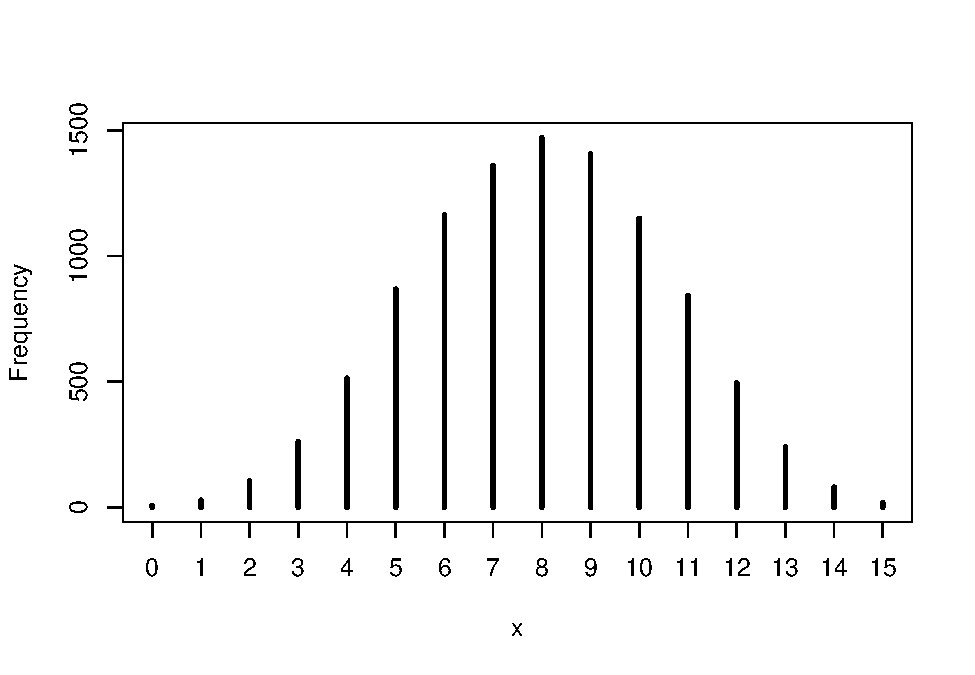
\includegraphics{03-samplingTheImaginary_files/figure-latex/unnamed-chunk-23-1.pdf}

\begin{Shaded}
\begin{Highlighting}[]
\NormalTok{prob_}\DecValTok{8}\NormalTok{_}\DecValTok{15}\NormalTok{ =}\StringTok{ }\KeywordTok{sum}\NormalTok{(w }\OperatorTok{==}\StringTok{ }\DecValTok{8}\NormalTok{)}\OperatorTok{/}\KeywordTok{length}\NormalTok{(w)}
\KeywordTok{round}\NormalTok{(}\DecValTok{100}\OperatorTok{*}\NormalTok{prob_}\DecValTok{8}\NormalTok{_}\DecValTok{15}\NormalTok{, }\DecValTok{4}\NormalTok{)}
\end{Highlighting}
\end{Shaded}

\begin{verbatim}
## [1] 14.7
\end{verbatim}

\hypertarget{m4.}{%
\subsection{3M4.}\label{m4.}}

Using the posterior distribution constructed from the new (8/15) data, now calculate the probability of observing 6 water in 9 tosses.

\textbf{Solution}
Use the posterior from 3M1 as the prior for this run, with \texttt{n\_trials\ =\ 9} and \texttt{n\_water\ =\ 6}:

\begin{Shaded}
\begin{Highlighting}[]
\NormalTok{w =}\StringTok{ }\KeywordTok{rbinom}\NormalTok{( }\FloatTok{1e4}\NormalTok{, }\DataTypeTok{size=}\DecValTok{9}\NormalTok{, }\DataTypeTok{prob=}\NormalTok{samples)}
\KeywordTok{simplehist}\NormalTok{(w)}
\end{Highlighting}
\end{Shaded}

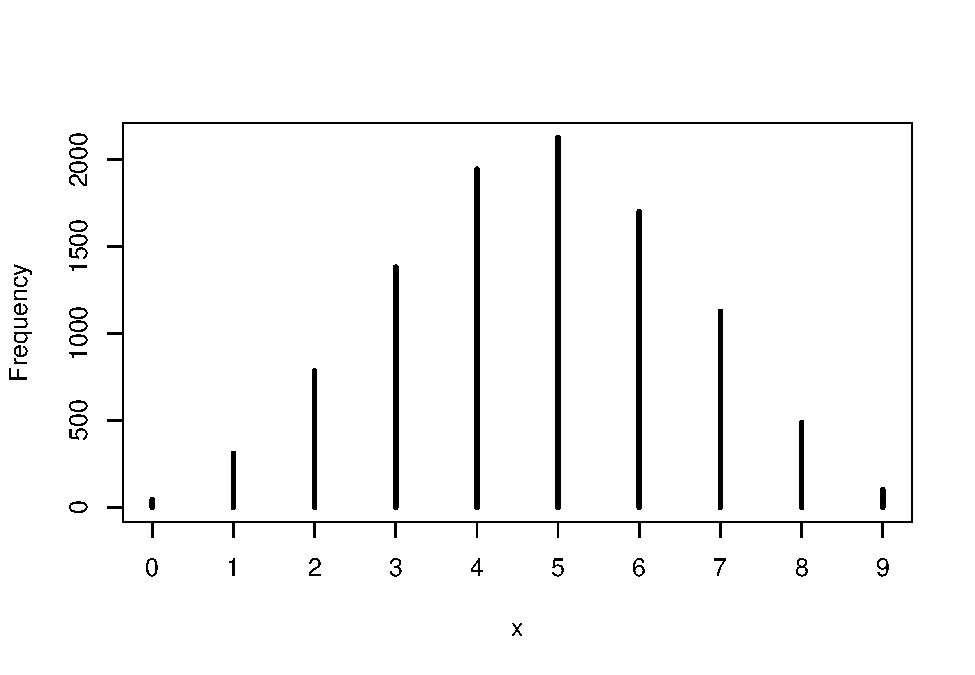
\includegraphics{03-samplingTheImaginary_files/figure-latex/unnamed-chunk-24-1.pdf}

\begin{Shaded}
\begin{Highlighting}[]
\NormalTok{prob_}\DecValTok{6}\NormalTok{_}\DecValTok{9}\NormalTok{ =}\StringTok{ }\KeywordTok{sum}\NormalTok{(w }\OperatorTok{==}\StringTok{ }\DecValTok{6}\NormalTok{)}\OperatorTok{/}\KeywordTok{length}\NormalTok{(w)}
\KeywordTok{round}\NormalTok{(}\DecValTok{100}\OperatorTok{*}\NormalTok{prob_}\DecValTok{6}\NormalTok{_}\DecValTok{9}\NormalTok{, }\DecValTok{4}\NormalTok{)}
\end{Highlighting}
\end{Shaded}

\begin{verbatim}
## [1] 17
\end{verbatim}

\hypertarget{m5.}{%
\subsection{3M5.}\label{m5.}}

Start over at 3M1, but now use a prior that is zero below p = 0.5 and a constant above p = 0.5. This corresponds to prior information that a majority of the Earth's surface is water. Repeat each problem above and compare the inferences. What difference does the better prior make? If it helps, compare inferences (using both priors) to the true value p = 0.7.

\textbf{Solution}
Simply pass a prior of the form \texttt{ifelse(\ p\_grid\ \textless{}\ 0.5,\ 0,\ 1)} instead of the uniform prior:

\begin{Shaded}
\begin{Highlighting}[]
\NormalTok{out2 =}\StringTok{ }\KeywordTok{globe_water_distn}\NormalTok{(}\DecValTok{15}\NormalTok{, }\DecValTok{8}\NormalTok{, }\DataTypeTok{prior =} \KeywordTok{ifelse}\NormalTok{(p_grid }\OperatorTok{<}\StringTok{ }\FloatTok{0.5}\NormalTok{, }\DecValTok{0}\NormalTok{, }\DecValTok{1}\NormalTok{))}

\NormalTok{n_samples =}\StringTok{ }\FloatTok{1e5}
\NormalTok{samples =}\StringTok{ }\KeywordTok{sample}\NormalTok{( out2[[}\StringTok{"p_grid"}\NormalTok{]], }
                  \DataTypeTok{size=}\NormalTok{n_samples, }
                  \DataTypeTok{replace=}\OtherTok{TRUE}\NormalTok{, }
                  \DataTypeTok{prob=}\NormalTok{out2[[}\StringTok{"posterior"}\NormalTok{]])}


\KeywordTok{plot}\NormalTok{( out2}\OperatorTok{$}\NormalTok{posterior }\OperatorTok{~}\StringTok{ }\NormalTok{out2}\OperatorTok{$}\NormalTok{p_grid, }\DataTypeTok{type =} \StringTok{"l"}\NormalTok{)}
\end{Highlighting}
\end{Shaded}

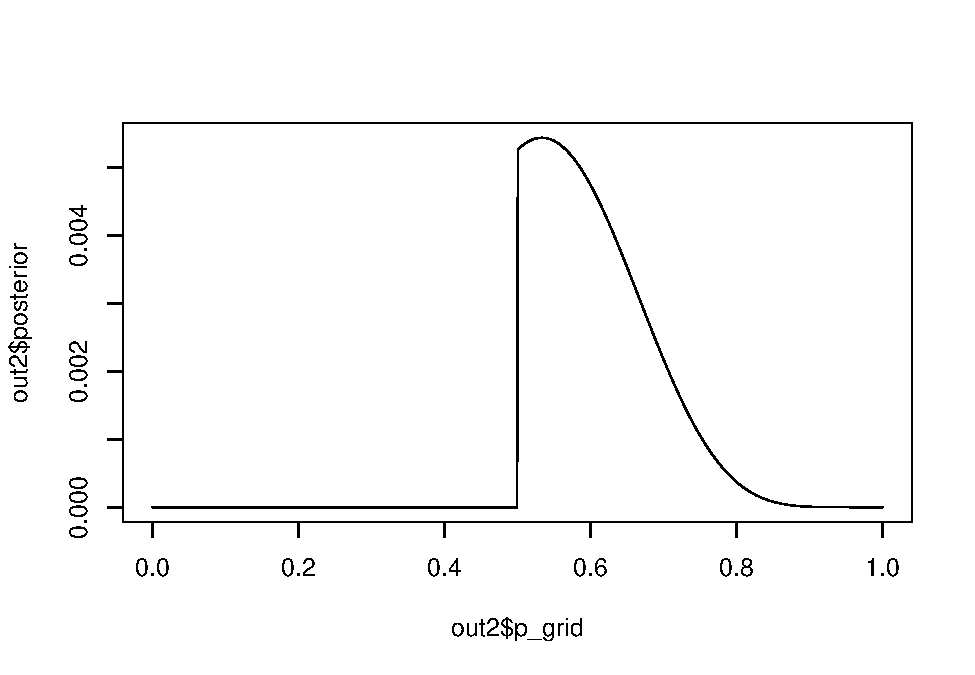
\includegraphics{03-samplingTheImaginary_files/figure-latex/unnamed-chunk-25-1.pdf}

\begin{Shaded}
\begin{Highlighting}[]
\NormalTok{hpdi90_}\DecValTok{2}\NormalTok{ =}\StringTok{ }\KeywordTok{HPDI}\NormalTok{( samples, }\DataTypeTok{prob =} \FloatTok{0.90}\NormalTok{)}
\NormalTok{hpdi90_}\DecValTok{2}
\end{Highlighting}
\end{Shaded}

\begin{verbatim}
##      |0.9      0.9| 
## 0.5005005 0.7117117
\end{verbatim}

\begin{Shaded}
\begin{Highlighting}[]
\KeywordTok{print}\NormalTok{(}\StringTok{"The uniform prior gave a 90% HPDI of:"}\NormalTok{)}
\end{Highlighting}
\end{Shaded}

\begin{verbatim}
## [1] "The uniform prior gave a 90% HPDI of:"
\end{verbatim}

\begin{Shaded}
\begin{Highlighting}[]
\KeywordTok{print}\NormalTok{(}\KeywordTok{round}\NormalTok{(hpdi90_}\DecValTok{1}\NormalTok{, }\DecValTok{2}\NormalTok{))}
\end{Highlighting}
\end{Shaded}

\begin{verbatim}
## |0.9 0.9| 
## 0.33 0.72
\end{verbatim}

\begin{Shaded}
\begin{Highlighting}[]
\KeywordTok{print}\NormalTok{(}\StringTok{"The informed prior gave a 90% HPDI of:"}\NormalTok{)}
\end{Highlighting}
\end{Shaded}

\begin{verbatim}
## [1] "The informed prior gave a 90% HPDI of:"
\end{verbatim}

\begin{Shaded}
\begin{Highlighting}[]
\KeywordTok{print}\NormalTok{(}\KeywordTok{round}\NormalTok{(hpdi90_}\DecValTok{2}\NormalTok{, }\DecValTok{2}\NormalTok{))}
\end{Highlighting}
\end{Shaded}

\begin{verbatim}
## |0.9 0.9| 
## 0.50 0.71
\end{verbatim}

\begin{Shaded}
\begin{Highlighting}[]
\KeywordTok{print}\NormalTok{(}\StringTok{"The informed prior leads to a narrower HPDI indicating that the informed prior leads to lesser uncertainty about the underlying value of the proportion of water on the globe's surface."}\NormalTok{)}
\end{Highlighting}
\end{Shaded}

\begin{verbatim}
## [1] "The informed prior leads to a narrower HPDI indicating that the informed prior leads to lesser uncertainty about the underlying value of the proportion of water on the globe's surface."
\end{verbatim}

Now the posterior predictive distribution:

\begin{Shaded}
\begin{Highlighting}[]
\NormalTok{w =}\StringTok{ }\KeywordTok{rbinom}\NormalTok{( }\FloatTok{1e4}\NormalTok{, }\DataTypeTok{size=}\DecValTok{15}\NormalTok{, }\DataTypeTok{prob=}\NormalTok{samples)}
\KeywordTok{simplehist}\NormalTok{(w)}
\end{Highlighting}
\end{Shaded}

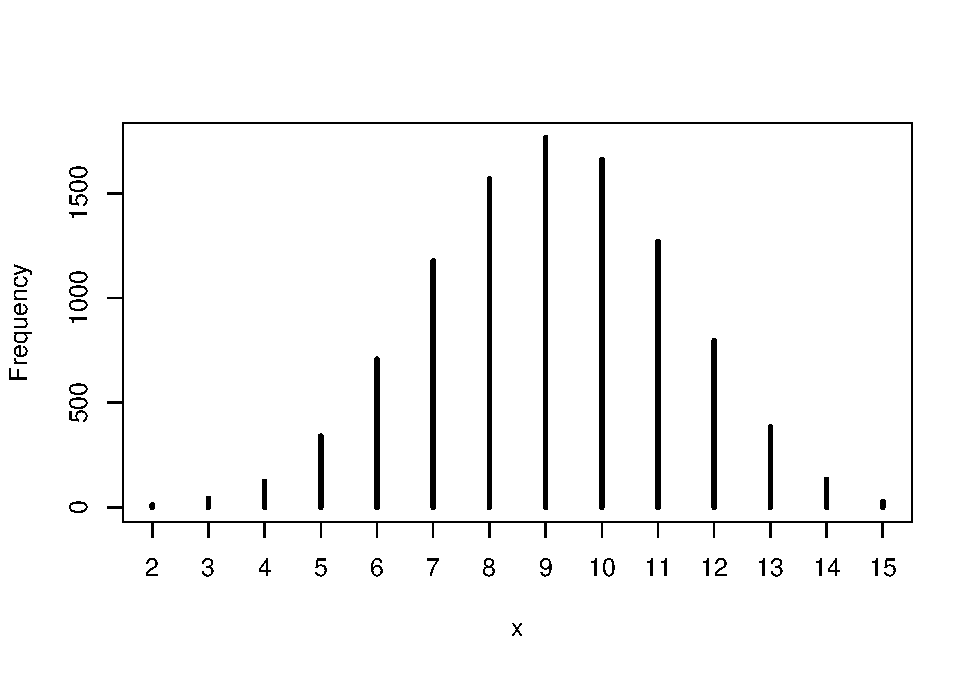
\includegraphics{03-samplingTheImaginary_files/figure-latex/unnamed-chunk-26-1.pdf}

\begin{Shaded}
\begin{Highlighting}[]
\NormalTok{prob_}\DecValTok{8}\NormalTok{_}\DecValTok{15}\NormalTok{ =}\StringTok{ }\KeywordTok{sum}\NormalTok{(w }\OperatorTok{==}\StringTok{ }\DecValTok{8}\NormalTok{)}\OperatorTok{/}\KeywordTok{length}\NormalTok{(w)}
\KeywordTok{round}\NormalTok{(}\DecValTok{100}\OperatorTok{*}\NormalTok{prob_}\DecValTok{8}\NormalTok{_}\DecValTok{15}\NormalTok{, }\DecValTok{4}\NormalTok{)}
\end{Highlighting}
\end{Shaded}

\begin{verbatim}
## [1] 15.69
\end{verbatim}

Now 8/15 is not exactly in the center of the posterior predictive distribution. The informative prior tells the model not to completely trust the data, so the simulated posterior sampling distributions are not quite centered on the data.

\hypertarget{m6.}{%
\subsection{3M6.}\label{m6.}}

Suppose you want to estimate the Earth's proportion of water very precisely. Specifically, you want the 99\% percentile interval of the posterior distribution of p to be only 0.05 wide. This means the distance between the upper and lower bound of the interval should be 0.05. How many times will you have to toss the globe to do this?

\textbf{Assuming the uniform prior}
Borrowed from \href{https://www.briancallander.com/posts/statistical-rethinking-2/exercise_3m}{Brian Callander} and done using tidyverse functions:

Bayesian models are generative, so we can simulate new datasets according to our prior probabilities. We'll simulate 100 datasets for each value of \(N\) of interest. We simulate a dataset by choosing a \texttt{p\_true} from our prior, then randomly choosing a \texttt{w} from the corresponding binomial distribution.

\begin{Shaded}
\begin{Highlighting}[]
\NormalTok{pacman}\OperatorTok{::}\KeywordTok{p_load}\NormalTok{(tidyverse)}
\NormalTok{m6_prior_predictive =}\StringTok{ }\KeywordTok{crossing}\NormalTok{(}
    \DataTypeTok{N =} \DecValTok{200} \OperatorTok{*}\StringTok{ }\NormalTok{(}\DecValTok{1}\OperatorTok{:}\DecValTok{16}\NormalTok{),}
    \DataTypeTok{iter =} \DecValTok{1}\OperatorTok{:}\DecValTok{10}
\NormalTok{) }\OperatorTok
\StringTok{    }\KeywordTok{mutate}\NormalTok{(}
        \DataTypeTok{p_true =} \KeywordTok{runif}\NormalTok{(}\KeywordTok{n}\NormalTok{(), }\DataTypeTok{min=}\DecValTok{0}\NormalTok{, }\DataTypeTok{max=}\DecValTok{1}\NormalTok{),}
        \DataTypeTok{W =} \KeywordTok{rbinom}\NormalTok{(}\KeywordTok{n}\NormalTok{(), N, p_true)}
\NormalTok{    )}
\end{Highlighting}
\end{Shaded}

For each of these simulated datasets, we grid approximate the posterior, take posterior samples, then calculate the HPDI

\begin{Shaded}
\begin{Highlighting}[]
\NormalTok{granularity =}\StringTok{ }\DecValTok{1000}
\NormalTok{m6_grid =}\StringTok{ }\KeywordTok{tibble}\NormalTok{(}\DataTypeTok{p =} \KeywordTok{seq}\NormalTok{(}\DecValTok{0}\NormalTok{, }\DecValTok{1}\NormalTok{, }\DataTypeTok{length.out =}\NormalTok{ granularity)) }\OperatorTok
\StringTok{    }\KeywordTok{mutate}\NormalTok{(}\DataTypeTok{prior =} \DecValTok{1}\NormalTok{)}

\NormalTok{m6_posteriors =}\StringTok{ }\NormalTok{m6_prior_predictive }\OperatorTok
\StringTok{    }\KeywordTok{crossing}\NormalTok{(m6_grid) }\OperatorTok
\StringTok{    }\KeywordTok{group_by}\NormalTok{(N, p_true, iter) }\OperatorTok
\StringTok{    }\KeywordTok{mutate}\NormalTok{(}
        \DataTypeTok{likelihood =} \KeywordTok{dbinom}\NormalTok{(W, N, p),}
        \DataTypeTok{posterior =}\NormalTok{ prior }\OperatorTok{*}\StringTok{ }\NormalTok{likelihood}
\NormalTok{    )}

\NormalTok{m6_samples =}\StringTok{ }\NormalTok{m6_posteriors }\OperatorTok
\StringTok{    }\KeywordTok{sample_n}\NormalTok{(}\DecValTok{1000}\NormalTok{, }\DataTypeTok{replace=}\OtherTok{TRUE}\NormalTok{, }\DataTypeTok{weight=}\NormalTok{posterior)}

\NormalTok{m6_hpdi =}\StringTok{ }\NormalTok{m6_samples }\OperatorTok
\StringTok{    }\KeywordTok{summarise}\NormalTok{(}\DataTypeTok{lo =} \KeywordTok{HPDI}\NormalTok{(p, }\FloatTok{0.99}\NormalTok{)[}\DecValTok{1}\NormalTok{], }\DataTypeTok{hi =} \KeywordTok{HPDI}\NormalTok{(p, }\FloatTok{0.99}\NormalTok{)[}\DecValTok{2}\NormalTok{]) }\OperatorTok
\StringTok{    }\KeywordTok{mutate}\NormalTok{(}\DataTypeTok{width =} \KeywordTok{abs}\NormalTok{(hi }\OperatorTok{-}\StringTok{ }\NormalTok{lo))}
\end{Highlighting}
\end{Shaded}

\begin{verbatim}
## `summarise()` regrouping output by 'N', 'p_true' (override with `.groups` argument)
\end{verbatim}

Now for each value of N, we check how many of the intervals have the desired width:

\begin{Shaded}
\begin{Highlighting}[]
\NormalTok{m6_n =}\StringTok{ }\NormalTok{m6_hpdi }\OperatorTok
\StringTok{    }\KeywordTok{group_by}\NormalTok{(N) }\OperatorTok
\StringTok{    }\KeywordTok{summarise}\NormalTok{(}\DataTypeTok{fraction =} \KeywordTok{mean}\NormalTok{(width }\OperatorTok{<}\StringTok{ }\FloatTok{0.05}\NormalTok{))}
\end{Highlighting}
\end{Shaded}

\begin{verbatim}
## `summarise()` ungrouping output (override with `.groups` argument)
\end{verbatim}

\begin{Shaded}
\begin{Highlighting}[]
\NormalTok{gg1 =}\StringTok{ }\KeywordTok{ggplot}\NormalTok{(}\DataTypeTok{data =}\NormalTok{ m6_n,}
             \DataTypeTok{mapping =} \KeywordTok{aes}\NormalTok{(}\DataTypeTok{x =}\NormalTok{ N, }\DataTypeTok{y =} \DecValTok{100} \OperatorTok{*}\StringTok{ }\NormalTok{fraction)) }\OperatorTok{+}
\StringTok{    }\KeywordTok{geom_point}\NormalTok{() }\OperatorTok{+}
\StringTok{    }\KeywordTok{geom_line}\NormalTok{()}

\NormalTok{gg1}
\end{Highlighting}
\end{Shaded}

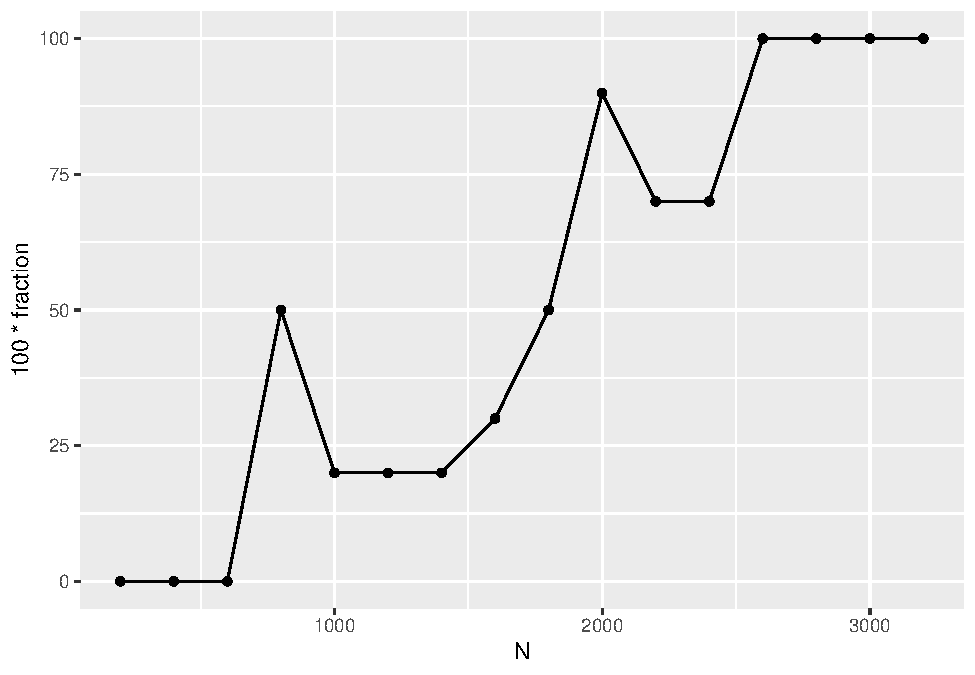
\includegraphics{03-samplingTheImaginary_files/figure-latex/unnamed-chunk-29-1.pdf}

\textbf{NB.} The hard problems here all use the data below. These data indicate the gender (male=1, female=0) of officially reported first and second born children in 100 two-child families. The data is in the \texttt{homeworkch3} data set:

\begin{Shaded}
\begin{Highlighting}[]
\NormalTok{pacman}\OperatorTok{::}\KeywordTok{p_load}\NormalTok{(rethinking)}
\KeywordTok{data}\NormalTok{(homeworkch3)}

\NormalTok{df =}\StringTok{ }\KeywordTok{tibble}\NormalTok{(}
    \DataTypeTok{birth1 =}\NormalTok{ birth1,}
    \DataTypeTok{birth2 =}\NormalTok{ birth2}
\NormalTok{) }\OperatorTok
\StringTok{    }\KeywordTok{mutate}\NormalTok{(}\DataTypeTok{family =} \KeywordTok{row_number}\NormalTok{())}
\end{Highlighting}
\end{Shaded}

\hypertarget{h1.}{%
\subsection{3H1.}\label{h1.}}

Using grid approximation, compute the posterior distribution for the probability of a birth being a boy. Assume a uniform prior probability. Which parameter value maximizes the posterior probability?

** Data story**

\begin{enumerate}
\def\labelenumi{\arabic{enumi}.}
\tightlist
\item
  The true proportion of boys births in 2-child families is \(p\)
\item
  A single sample of a 2-child family has probability \(p\) of having a boy birth, and probaility \(1-p\) of having a not boy (girl) birth.
\item
  Each family sampled is independent of the others, and each birth within a family is independent in terms of propensity for a particular gender (this may not be quite valid).
\end{enumerate}

\textbf{Model}

Let \(B\) denote the number of boy births and \(G\) denote the number of girl births, and assign the data model:
\[
 B \sim \text{Binomial}(N,p)
\]
where \(N = B + G\). Suppose we have vague prior information and assume it is uniform:
\[
p \sim \text{Uniform}(0,1)
\]
Then we can in this case, \(N=200\) (2 children in each of 100 families).

Let's check the total number of boys and girls:

\begin{Shaded}
\begin{Highlighting}[]
\NormalTok{h1_birthcounts =}\StringTok{ }\NormalTok{df }\OperatorTok
\StringTok{    }\KeywordTok{summarise}\NormalTok{(}
        \DataTypeTok{boy_births =} \KeywordTok{sum}\NormalTok{(}\KeywordTok{c}\NormalTok{(birth1, birth2)),}
        \DataTypeTok{total_births =} \KeywordTok{length}\NormalTok{(}\KeywordTok{c}\NormalTok{(birth1, birth2))}
\NormalTok{    )}
\NormalTok{h1_birthcounts}
\end{Highlighting}
\end{Shaded}

\begin{verbatim}
## # A tibble: 1 x 2
##   boy_births total_births
##        <dbl>        <int>
## 1        111          200
\end{verbatim}

Now proceed to a grid-approximation of the posterior

\begin{Shaded}
\begin{Highlighting}[]
\CommentTok{# define global variables}
\NormalTok{granularity =}\StringTok{ }\DecValTok{1000}

\CommentTok{# define grid}
\NormalTok{h1_p_grid =}\StringTok{ }\KeywordTok{tibble}\NormalTok{(}\DataTypeTok{p =} \KeywordTok{seq}\NormalTok{( }\DataTypeTok{from=}\DecValTok{0}\NormalTok{, }\DataTypeTok{to=}\DecValTok{1}\NormalTok{, }\DataTypeTok{length.out=}\NormalTok{granularity)) }\OperatorTok
\StringTok{    }\KeywordTok{mutate}\NormalTok{(}\DataTypeTok{prior =} \DecValTok{1}\NormalTok{)}

\CommentTok{# grid-approximation of posterior}
\NormalTok{h1_posterior =}\StringTok{ }\NormalTok{h1_p_grid }\OperatorTok
\StringTok{    }\KeywordTok{mutate}\NormalTok{(}
        \DataTypeTok{likelihood =} \KeywordTok{dbinom}\NormalTok{(}
            \DataTypeTok{x =}\NormalTok{ h1_birthcounts}\OperatorTok{$}\NormalTok{boy_births,}
            \DataTypeTok{size =}\NormalTok{ h1_birthcounts}\OperatorTok{$}\NormalTok{total_births,}
            \DataTypeTok{prob =}\NormalTok{ p),}
        \DataTypeTok{posterior =}\NormalTok{ (prior }\OperatorTok{*}\StringTok{ }\NormalTok{likelihood)}\OperatorTok{/}\KeywordTok{sum}\NormalTok{(prior}\OperatorTok{*}\NormalTok{likelihood)}
\NormalTok{    )}
\end{Highlighting}
\end{Shaded}

The maximum \emph{a posteriori} (MAP) estimate is:

\begin{Shaded}
\begin{Highlighting}[]
\NormalTok{h1_map =}\StringTok{ }\NormalTok{h1_posterior }\OperatorTok
\StringTok{    }\KeywordTok{slice}\NormalTok{(}\KeywordTok{which.max}\NormalTok{(posterior)) }\OperatorTok
\StringTok{    }\KeywordTok{pull}\NormalTok{(p)}

\NormalTok{h1_map }\OperatorTok\StringTok{ }\KeywordTok{round}\NormalTok{(}\DecValTok{2}\NormalTok{)}
\end{Highlighting}
\end{Shaded}

\begin{verbatim}
## [1] 0.55
\end{verbatim}

Create a plot to show this:

\begin{Shaded}
\begin{Highlighting}[]
\NormalTok{h1_ggp =}\StringTok{ }\NormalTok{h1_posterior }\OperatorTok
\StringTok{    }\KeywordTok{ggplot}\NormalTok{( }\KeywordTok{aes}\NormalTok{(}\DataTypeTok{x =}\NormalTok{ p) ) }\OperatorTok{+}
\StringTok{    }\KeywordTok{geom_line}\NormalTok{( }\KeywordTok{aes}\NormalTok{(}\DataTypeTok{y =}\NormalTok{ posterior) ) }\OperatorTok{+}\StringTok{ }
\StringTok{    }\KeywordTok{geom_area}\NormalTok{( }\KeywordTok{aes}\NormalTok{(}\DataTypeTok{y =}\NormalTok{ posterior), }\DataTypeTok{colour=}\StringTok{"white"}\NormalTok{, }\DataTypeTok{fill=}\StringTok{"steelblue"}\NormalTok{ )}


\NormalTok{h1_ggp }\OperatorTok{+}\StringTok{ }\KeywordTok{geom_vline}\NormalTok{(}\KeywordTok{aes}\NormalTok{(}\DataTypeTok{xintercept =}\NormalTok{ h1_map),}
               \DataTypeTok{color=}\StringTok{"red"}\NormalTok{,}
               \DataTypeTok{linetype=}\StringTok{"dashed"}\NormalTok{,}
               \DataTypeTok{size=}\DecValTok{1}\NormalTok{) }\OperatorTok{+}
\StringTok{    }\KeywordTok{annotate}\NormalTok{(}\DataTypeTok{geom =} \StringTok{"text"}\NormalTok{,}
             \DataTypeTok{x =} \FloatTok{0.65}\NormalTok{, }\DataTypeTok{y =} \FloatTok{0.012}\NormalTok{,}
             \DataTypeTok{label =} \KeywordTok{paste}\NormalTok{(}\StringTok{"MAP ="}\NormalTok{, h1_map }\OperatorTok\StringTok{ }\KeywordTok{round}\NormalTok{(}\DecValTok{2}\NormalTok{)),}
             \DataTypeTok{color=}\StringTok{"red"}\NormalTok{) }\OperatorTok{+}
\StringTok{    }\KeywordTok{labs}\NormalTok{(}\DataTypeTok{x =} \StringTok{"Probability of a boy birth (p)"}\NormalTok{,}
         \DataTypeTok{y =} \StringTok{"Probability Density"}\NormalTok{,}
         \DataTypeTok{title =} \StringTok{"3H1 Posterior probability of giving birth to a boy"}\NormalTok{) }\OperatorTok{+}
\StringTok{    }\KeywordTok{theme_minimal}\NormalTok{()}
\end{Highlighting}
\end{Shaded}

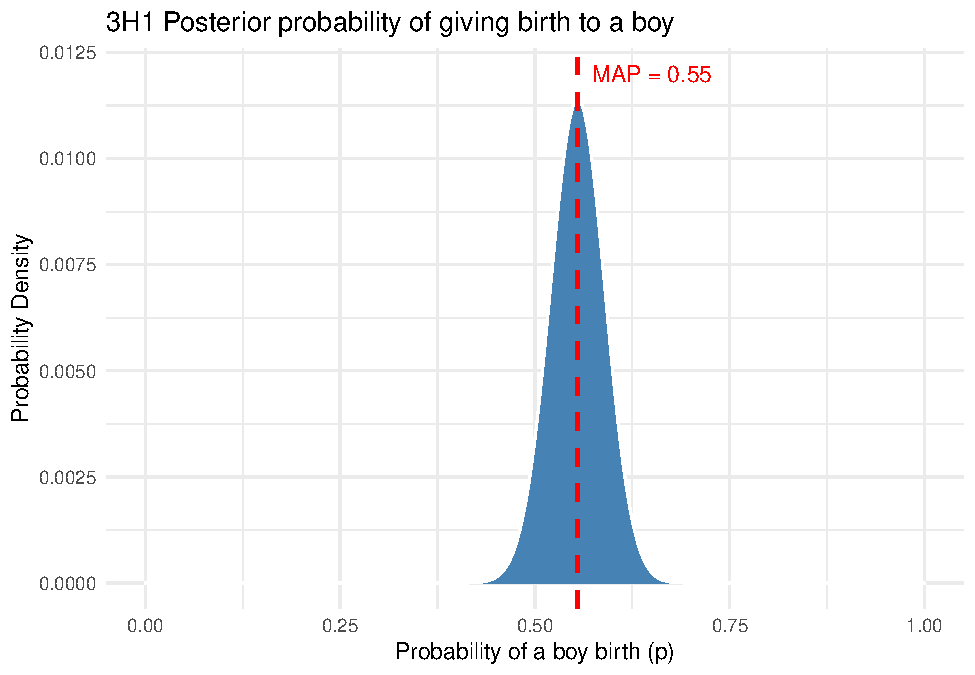
\includegraphics{03-samplingTheImaginary_files/figure-latex/unnamed-chunk-34-1.pdf}

\hypertarget{h2.}{%
\subsection{3H2.}\label{h2.}}

Using the sample function, draw 10,000 random parameter values from the posterior distribution you calculated above. Use these samples to estimate the 50\%, 89\%, and 97\% highest posterior density intervals.

\textbf{Solution}

Draw samples from the grid weighted according to the posterior probabilities. Can do this following the book as:

\begin{Shaded}
\begin{Highlighting}[]
\CommentTok{# rethinking approach:}
\NormalTok{n_samples =}\StringTok{ }\FloatTok{1e4}
\NormalTok{h2_samples =}\StringTok{ }\KeywordTok{with}\NormalTok{(h1_posterior, }
               \KeywordTok{sample}\NormalTok{(p, }\DataTypeTok{prob =}\NormalTok{ posterior, }\DataTypeTok{size=}\NormalTok{n_samples, }\DataTypeTok{replace=}\OtherTok{TRUE}\NormalTok{) )}
\end{Highlighting}
\end{Shaded}

and then use \texttt{rethinking::HPDI()} to find highest posterior density intervals for the given levels. However, we can also use a \texttt{tidyverse} approach:

\begin{Shaded}
\begin{Highlighting}[]
\CommentTok{# tidyverse approach:}
\NormalTok{n_samples =}\StringTok{ }\FloatTok{1e4}
\NormalTok{h2_samples =}\StringTok{ }\NormalTok{h1_posterior }\OperatorTok
\StringTok{    }\KeywordTok{sample_n}\NormalTok{(}\DataTypeTok{size =}\NormalTok{ n_samples, }\DataTypeTok{replace=}\OtherTok{TRUE}\NormalTok{, }\DataTypeTok{weight=}\NormalTok{posterior) }\OperatorTok
\StringTok{    }\KeywordTok{pull}\NormalTok{(p)}

\NormalTok{h2_hpdi =}\StringTok{ }\NormalTok{h2_samples }\OperatorTok
\StringTok{    }\KeywordTok{crossing}\NormalTok{(}\DataTypeTok{prob =} \KeywordTok{c}\NormalTok{(}\FloatTok{0.5}\NormalTok{, }\FloatTok{0.89}\NormalTok{, }\FloatTok{0.97}\NormalTok{)) }\OperatorTok
\StringTok{    }\KeywordTok{group_by}\NormalTok{(prob) }\OperatorTok
\StringTok{    }\KeywordTok{group_map}\NormalTok{(HPDI)}

\NormalTok{h2_hpdi}
\end{Highlighting}
\end{Shaded}

\begin{verbatim}
## [[1]]
##      |0.5      0.5| 
## 0.5005005 0.6126126 
## 
## [[2]]
##     |0.89     0.89| 
## 0.4534535 0.6516517 
## 
## [[3]]
##     |0.97     0.97| 
## 0.4454454 0.6746747
\end{verbatim}

\hypertarget{h3.}{%
\subsection{3H3.}\label{h3.}}

Use rbinom to simulate 10,000 replicates of 200 births. You should end up with 10,000 numbers, each one a count of boys out of 200 births. Compare the distribution of predicted numbers of boys to the actual count in the data (111 boys out of 200 births). There are many good ways to visualize the simulations, but the dens command (part of the rethinking package) is probably the easiest way in this case. Does it look like the model fits the data well? That is, does the distribution of predictions include the actual observation as a central, likely outcome?

\textbf{Solution}
Samples from the posterior predictive distribution are ``possible'' observed counts of boy births from 200 according to the posterior, and it's easy to generate these (under a uniform prior) by simply setting the \texttt{prob} argument of \texttt{rbinom()} to values in \texttt{h2\_samples}, to draw binomial random numbers as follows:

\begin{Shaded}
\begin{Highlighting}[]
\CommentTok{# posterior predictive samples}
\NormalTok{h3_posterior_predictive =}\StringTok{ }\KeywordTok{tibble}\NormalTok{(}
    \DataTypeTok{predicted_values =} \KeywordTok{rbinom}\NormalTok{(}\DataTypeTok{n=}\FloatTok{1e4}\NormalTok{, }\DataTypeTok{size=}\DecValTok{200}\NormalTok{, }\DataTypeTok{prob=}\NormalTok{h2_samples) )}

\CommentTok{# plot the posterior predictive distribution and }
\CommentTok{# draw a vertical line to indicate the actual observed value of 111 from 200.}
\NormalTok{h3_ggp =}\StringTok{ }\NormalTok{h3_posterior_predictive }\OperatorTok
\StringTok{    }\KeywordTok{ggplot}\NormalTok{( }\KeywordTok{aes}\NormalTok{(}\DataTypeTok{x =}\NormalTok{ predicted_values) ) }\OperatorTok{+}
\StringTok{    }\KeywordTok{geom_histogram}\NormalTok{(}\KeywordTok{aes}\NormalTok{(}\DataTypeTok{y=}\NormalTok{..density..), }\DataTypeTok{colour=}\StringTok{"black"}\NormalTok{, }\DataTypeTok{fill=}\StringTok{"cyan4"}\NormalTok{) }\OperatorTok{+}
\StringTok{    }\KeywordTok{geom_density}\NormalTok{( }\DataTypeTok{alpha=}\FloatTok{0.2}\NormalTok{, }\DataTypeTok{fill=}\StringTok{"cyan"}\NormalTok{) }\OperatorTok{+}
\StringTok{    }\KeywordTok{geom_vline}\NormalTok{(}\KeywordTok{aes}\NormalTok{(}\DataTypeTok{xintercept =}\NormalTok{ h1_birthcounts}\OperatorTok{$}\NormalTok{boy_births),}
               \DataTypeTok{color=}\StringTok{"darkorange"}\NormalTok{,}
               \DataTypeTok{linetype=}\StringTok{"dashed"}\NormalTok{,}
               \DataTypeTok{size=}\FloatTok{1.25}\NormalTok{) }\OperatorTok{+}
\StringTok{    }\KeywordTok{labs}\NormalTok{(}\DataTypeTok{x =} \StringTok{"Number of boys in 200 births"}\NormalTok{,}
         \DataTypeTok{y =} \StringTok{"Probability Density"}\NormalTok{,}
         \DataTypeTok{title =} \StringTok{"3H3: the posterior predictive distribution for 200 births"}\NormalTok{,}
         \DataTypeTok{subtitle =} \StringTok{"The dashed line indicates the actual data: 111 boys born from 200 births"}\NormalTok{) }\OperatorTok{+}
\StringTok{        }\KeywordTok{theme_minimal}\NormalTok{()}

\NormalTok{h3_ggp}
\end{Highlighting}
\end{Shaded}

\begin{verbatim}
## `stat_bin()` using `bins = 30`. Pick better value with `binwidth`.
\end{verbatim}

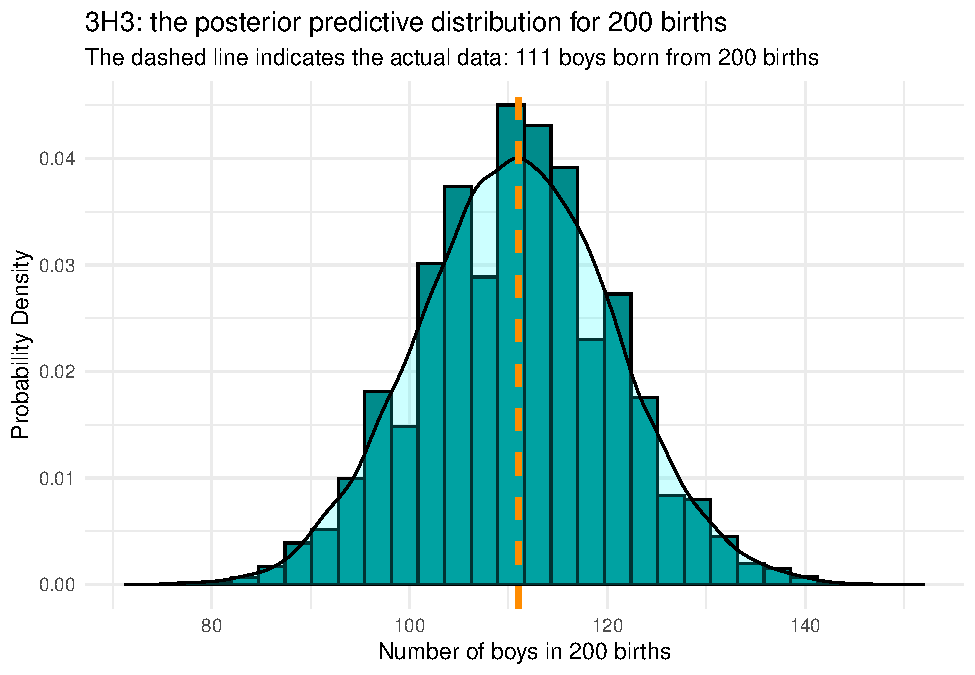
\includegraphics{03-samplingTheImaginary_files/figure-latex/unnamed-chunk-37-1.pdf}

As can be seen, the actual observed value of 111 boy births from 200 total births is very close to the peak of the posterior predictive distribution, so that indicates that our model is placing most probability in the region that the data indicates is appropriate.

\hypertarget{h4.}{%
\subsection{3H4.}\label{h4.}}

Now compare 10,000 counts of boys from 100 simulated first borns only to the number of boys in the first births, birth1. How does the model look in this light?

\textbf{Solution}
So far we've considered getting 111 from 200 births, but these come from only 100 families, and we've so far ignored any influence of birth order. But we can easily produce a new predictive distribution that only deals with the first 100 births (i.e.~the first births in each family):

\begin{Shaded}
\begin{Highlighting}[]
\CommentTok{# posterior predictive samples}
\NormalTok{h4_posterior_predictive =}\StringTok{ }\KeywordTok{tibble}\NormalTok{(}
    \DataTypeTok{predicted_values =} \KeywordTok{rbinom}\NormalTok{(}\DataTypeTok{n=}\FloatTok{1e4}\NormalTok{, }\DataTypeTok{size=}\DecValTok{100}\NormalTok{, }\DataTypeTok{prob=}\NormalTok{h2_samples) )}

\CommentTok{# plot the posterior predictive distribution and }
\CommentTok{# draw a vertical line to indicate the actual observed value of 111 from 200.}
\NormalTok{h4_ggp =}\StringTok{ }\NormalTok{h4_posterior_predictive }\OperatorTok
\StringTok{    }\KeywordTok{ggplot}\NormalTok{( }\KeywordTok{aes}\NormalTok{(}\DataTypeTok{x =}\NormalTok{ predicted_values) ) }\OperatorTok{+}
\StringTok{    }\KeywordTok{geom_histogram}\NormalTok{(}\KeywordTok{aes}\NormalTok{(}\DataTypeTok{y=}\NormalTok{..density..), }\DataTypeTok{colour=}\StringTok{"black"}\NormalTok{, }\DataTypeTok{fill=}\StringTok{"cyan4"}\NormalTok{) }\OperatorTok{+}
\StringTok{    }\KeywordTok{geom_density}\NormalTok{( }\DataTypeTok{alpha=}\FloatTok{0.2}\NormalTok{, }\DataTypeTok{fill=}\StringTok{"cyan"}\NormalTok{) }\OperatorTok{+}
\StringTok{    }\KeywordTok{geom_vline}\NormalTok{(}\KeywordTok{aes}\NormalTok{(}\DataTypeTok{xintercept =} \KeywordTok{sum}\NormalTok{(df}\OperatorTok{$}\NormalTok{birth1)),}
               \DataTypeTok{color=}\StringTok{"darkorange"}\NormalTok{,}
               \DataTypeTok{linetype=}\StringTok{"dashed"}\NormalTok{,}
               \DataTypeTok{size=}\FloatTok{1.25}\NormalTok{) }\OperatorTok{+}
\StringTok{    }\KeywordTok{labs}\NormalTok{(}\DataTypeTok{x =} \StringTok{"Number of boys in 100 births"}\NormalTok{,}
         \DataTypeTok{y =} \StringTok{"Probability Density"}\NormalTok{,}
         \DataTypeTok{title =} \StringTok{"3H4: the posterior predictive distribution for 100 births"}\NormalTok{,}
         \DataTypeTok{subtitle =} \StringTok{"The dashed line indicates the actual data: 51 boys born from 100 first-born births"}\NormalTok{) }\OperatorTok{+}
\StringTok{        }\KeywordTok{theme_minimal}\NormalTok{()}

\NormalTok{h4_ggp}
\end{Highlighting}
\end{Shaded}

\begin{verbatim}
## `stat_bin()` using `bins = 30`. Pick better value with `binwidth`.
\end{verbatim}

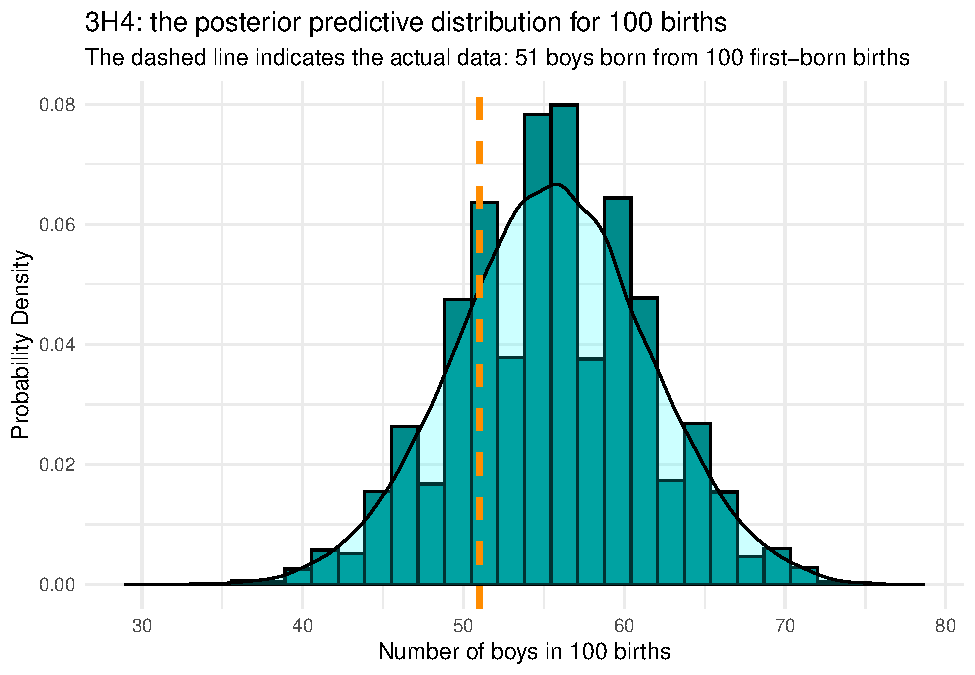
\includegraphics{03-samplingTheImaginary_files/figure-latex/unnamed-chunk-38-1.pdf}

\begin{Shaded}
\begin{Highlighting}[]
\CommentTok{## What's the probability of between 50 and 52 first births under the posterior ## predictive distribution?}
\NormalTok{h4_posterior_predictive }\OperatorTok
\StringTok{    }\KeywordTok{summarise}\NormalTok{(}\DataTypeTok{prob_51_100 =} \DecValTok{100}\OperatorTok{*}\KeywordTok{mean}\NormalTok{(predicted_values }\OperatorTok{>}\StringTok{ }\DecValTok{50} \OperatorTok{&}\StringTok{ }\NormalTok{predicted_values }\OperatorTok{<}\StringTok{ }\DecValTok{52}\NormalTok{))}
\end{Highlighting}
\end{Shaded}

\begin{verbatim}
## # A tibble: 1 x 1
##   prob_51_100
##         <dbl>
## 1        5.14
\end{verbatim}

\begin{Shaded}
\begin{Highlighting}[]
\CommentTok{## What's the achieved level of significance}
\NormalTok{h4_posterior_predictive }\OperatorTok
\StringTok{    }\KeywordTok{summarise}\NormalTok{(}\DataTypeTok{prob_als51_100 =} \DecValTok{100}\OperatorTok{*}\KeywordTok{mean}\NormalTok{(predicted_values }\OperatorTok{<=}\StringTok{ }\DecValTok{51}\NormalTok{))}
\end{Highlighting}
\end{Shaded}

\begin{verbatim}
## # A tibble: 1 x 1
##   prob_als51_100
##            <dbl>
## 1           25.2
\end{verbatim}

\begin{Shaded}
\begin{Highlighting}[]
\CommentTok{## What's the MAP estimate for the predictive distribution}
\NormalTok{h4_dens =}\StringTok{ }\KeywordTok{with}\NormalTok{(h4_posterior_predictive,}
               \KeywordTok{density}\NormalTok{(predicted_values))}

\NormalTok{h4_dens}\OperatorTok{$}\NormalTok{x[ }\KeywordTok{which.max}\NormalTok{(h4_dens}\OperatorTok{$}\NormalTok{y) ]}
\end{Highlighting}
\end{Shaded}

\begin{verbatim}
## [1] 55.71489
\end{verbatim}

Now the fit of the model doesn't look quite so good. It's not terrible, but the model MAP estimated number of first-born boys being about 55, and values of 51 or fewer are only expected about \(25\%\) of the time. From the predicted values, we only expect to observe 51 first-born male births slightly less than \(5\%\) of the time.

\hypertarget{h5.}{%
\subsection{3H5.}\label{h5.}}

The model assumes that sex of first and second births are independent. To check this assumption, focus now on second births that followed female first borns. Compare 10,000 simulated counts of boys to only those second births that followed girls. To do this correctly, you need to count the number of first borns who were girls and simulate that many births, 10,000 times. Compare the counts of boys in your simulations to the actual observed count of boys following girls. How does the model look in this light? Any guesses what is going on in these data?

\textbf{Solution}
Let's check the number of boys born after a girl.

\begin{Shaded}
\begin{Highlighting}[]
\NormalTok{h5_birthcounts =}\StringTok{ }\NormalTok{df }\OperatorTok
\StringTok{    }\KeywordTok{filter}\NormalTok{(birth1 }\OperatorTok{==}\StringTok{ }\DecValTok{0}\NormalTok{) }\OperatorTok
\StringTok{    }\KeywordTok{summarise}\NormalTok{(}\DataTypeTok{boy_births =} \KeywordTok{sum}\NormalTok{(birth2), }\DataTypeTok{total_births =} \KeywordTok{n}\NormalTok{())}

\NormalTok{h5_posterior_predictive =}\StringTok{ }\KeywordTok{tibble}\NormalTok{(}
    \DataTypeTok{predicted_values =} \KeywordTok{rbinom}\NormalTok{(}
        \DataTypeTok{n =} \FloatTok{1e4}\NormalTok{, }
        \DataTypeTok{size =}\NormalTok{ h5_birthcounts}\OperatorTok{$}\NormalTok{boy_births,}
        \DataTypeTok{prob =}\NormalTok{ h2_samples)}
\NormalTok{)}

\NormalTok{h5_ggp =}\StringTok{ }\NormalTok{h5_posterior_predictive }\OperatorTok
\StringTok{    }\KeywordTok{ggplot}\NormalTok{( }\KeywordTok{aes}\NormalTok{(}\DataTypeTok{x =}\NormalTok{ predicted_values) ) }\OperatorTok{+}
\StringTok{    }\KeywordTok{geom_histogram}\NormalTok{(}\KeywordTok{aes}\NormalTok{(}\DataTypeTok{y=}\NormalTok{..density..), }\DataTypeTok{colour=}\StringTok{"black"}\NormalTok{, }\DataTypeTok{fill=}\StringTok{"cyan4"}\NormalTok{) }\OperatorTok{+}
\StringTok{    }\KeywordTok{geom_density}\NormalTok{( }\DataTypeTok{alpha=}\FloatTok{0.2}\NormalTok{, }\DataTypeTok{fill=}\StringTok{"cyan"}\NormalTok{) }\OperatorTok{+}
\StringTok{    }\KeywordTok{geom_vline}\NormalTok{(}\KeywordTok{aes}\NormalTok{(}\DataTypeTok{xintercept =}\NormalTok{ h5_birthcounts}\OperatorTok{$}\NormalTok{boy_births),}
               \DataTypeTok{color=}\StringTok{"darkorange"}\NormalTok{,}
               \DataTypeTok{linetype=}\StringTok{"dashed"}\NormalTok{,}
               \DataTypeTok{size=}\FloatTok{1.25}\NormalTok{) }\OperatorTok{+}
\StringTok{    }\KeywordTok{labs}\NormalTok{(}\DataTypeTok{x =} \StringTok{"Number of 2nd-born boys after female 1st-borns"}\NormalTok{,}
         \DataTypeTok{y =} \StringTok{"Probability Density"}\NormalTok{,}
         \DataTypeTok{title =} \StringTok{"3H5: the posterior predictive distribution"}\NormalTok{,}
         \DataTypeTok{subtitle =} \StringTok{"The dashed line indicates the actual data: 39 boys born following after 49 first-born girls"}\NormalTok{) }\OperatorTok{+}
\StringTok{        }\KeywordTok{theme_minimal}\NormalTok{()}

\NormalTok{h5_ggp}
\end{Highlighting}
\end{Shaded}

\begin{verbatim}
## `stat_bin()` using `bins = 30`. Pick better value with `binwidth`.
\end{verbatim}

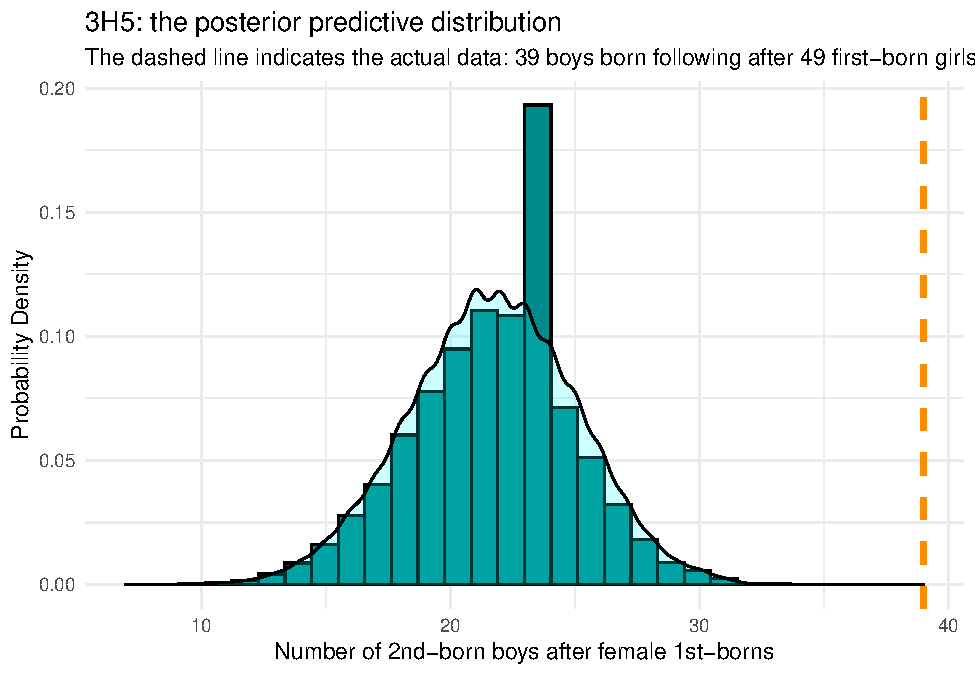
\includegraphics{03-samplingTheImaginary_files/figure-latex/unnamed-chunk-39-1.pdf}

\begin{Shaded}
\begin{Highlighting}[]
\CommentTok{## What's the achieved level of significance}
\NormalTok{h5_posterior_predictive }\OperatorTok
\StringTok{    }\KeywordTok{summarise}\NormalTok{(}\DataTypeTok{prob_als39_49 =} \DecValTok{100}\OperatorTok{*}\KeywordTok{mean}\NormalTok{(predicted_values }\OperatorTok{>=}\StringTok{ }\DecValTok{39}\NormalTok{))}
\end{Highlighting}
\end{Shaded}

\begin{verbatim}
## # A tibble: 1 x 1
##   prob_als39_49
##           <dbl>
## 1             0
\end{verbatim}

The fit here is very poor, indicating that the assumption of independence of birth gender from first born to second born is not adequate. Indeed, none of the 10000 predicted observations were as high as 39 second-born male births following on from 49 first-born female births. We should stratify this model and fit to first and then second and make that distinction the whole way through.

  \bibliography{book.bib}

\end{document}
